% Paper 1 schematic: sections, key equations, figures, barest writing.
% Figures and circuit macros are local copies (figures/, see figures/SOURCES.md) of the thesis chapter draft
% (../qsvt_thesis_chapter_draft/), which is the supporting note. The folder is self-contained for Overleaf.
\documentclass[11pt,a4paper]{article}
\usepackage[T1]{fontenc}\usepackage[utf8]{inputenc}\usepackage{lmodern}
\usepackage[margin=2.2cm]{geometry}
\usepackage{amsmath,amssymb}\usepackage{booktabs}\usepackage{graphicx}
\usepackage[labelfont=bf,font=small,skip=4pt]{caption}
\usepackage{float}\usepackage{xcolor}\usepackage{tikz}
\usetikzlibrary{decorations.pathreplacing,calc}
% TikZ styles and helpers shared by figures/circuits.tex and figures/circuits_qsvt.tex
\tikzset{
  wire/.style={line width=0.55pt},
  gate/.style={draw,fill=white,minimum height=6.2mm,minimum width=7.5mm,inner sep=1.5pt,font=\small,line width=0.55pt},
  wgate/.style={gate,minimum width=13mm},
  ctrl/.style={circle,fill=black,inner sep=0pt,minimum size=1.9mm},
  octrl/.style={circle,draw,fill=white,inner sep=0pt,minimum size=1.9mm,line width=0.55pt},
  targ/.style={circle,draw,inner sep=0pt,minimum size=3.2mm,line width=0.55pt},
  meter/.style={draw,fill=white,minimum height=6.2mm,minimum width=7.5mm,line width=0.55pt},
  reg/.style={font=\small,anchor=east},
  blk/.style={font=\footnotesize,anchor=north,text=black!65},
  st/.style={font=\footnotesize,anchor=south,text=blue!45!black},
  brace/.style={decorate,decoration={brace,mirror,amplitude=2.2pt},line width=0.4pt,black!60},
  slash/.style={},
}
\newcommand{\slashwire}[3]{% x y label : the /n mark on a multi-qubit wire
  \draw[line width=0.7pt] (#1cm-1.3mm,#2cm-1.6mm) -- (#1cm+1.3mm,#2cm+1.6mm);
  \node[font=\scriptsize,anchor=south west,inner sep=0.4pt] at (#1cm+0.9mm,#2cm+0.9mm) {#3};}
\newcommand{\vsep}[3]{% x ybot ytop : a dashed block boundary
  \draw[dashed,black!45,line width=0.4pt] (#1cm,#2cm) -- (#1cm,#3cm);}


\usepackage{parskip}\usepackage{enumitem}
\usepackage[colorlinks=true,linkcolor=blue!60!black,urlcolor=blue!70!black]{hyperref}
\graphicspath{{figures/}}
\newcommand{\eff}{\ensuremath{\varepsilon_{\rm seg}}}
\newcommand{\far}{\ensuremath{f_{\rm seg}}}
\newcommand{\msg}[1]{\noindent\textit{\color{blue!50!black}#1}\par\medskip}
\newcommand{\src}[1]{{\footnotesize\color{gray}#1}}
\title{\vspace{-1.5cm}From one bit to any polynomial:\\ QSVT spectral filters for track finding in the LHCb VELO toy\\[4pt]
\large Schematic of paper 1 --- sections, key equations, figures}
\author{G.\,W.\,Scriven (Maastricht, Hasselt, Nikhef)\\ \normalsize with X.\,Chiotopoulos, D.\,Nicotra, J.\,Sch\"utz, J.\,de Vries, M.\,Merk (author list to be agreed)}
\date{Schematic, 16 September 2026 (section 1 rebuilt on the paper corpus) --- target: Communications Physics, about 5{,}000 words, six figures, Methods, supplement}
\makeatletter
\newlabel{fig:circuits}{{1}{2}{}{}{}}
\newlabel{sec:fork:trotter}{{ch.\,11.4}{7}{}{}{}}
\makeatother
\begin{document}
\maketitle
\vspace{-8pt}
\msg{One sentence. The one-bit quantum filter's single zero removes the isolated false segments and nothing else; with more roots the same primitive removes the coupled ones; the price is depth per call, which a block encoding priced by detector hits converts into qubits.}
\src{Source of every figure and number: the thesis chapter draft \texttt{QSVT/Paper\_planning/qsvt\_thesis\_chapter\_draft/main.tex} (commit \texttt{c506a38b}); the figure ledger \texttt{QSVT/Efficiency\_Frontier/FIGURE\_DATA\_SOURCES.md}. Chapter sections are cited as [ch.~x.y].}

\section{Introduction}
\msg{Prose only. Tracking is a linear system; HHL was too deep and too slow to read out; the one-bit filter kept one bit to cut the readout, and pays for it in false segments; a polynomial keeps the efficiency and removes them.}
\begin{itemize}[leftmargin=1.5em,itemsep=2pt]
\item The problem: at the High-Luminosity LHC the candidate segments grow as $T^2$, the real ones as $T$: $n_{\rm seg}=4T^2$, $n_{\rm true}=4T$.
\item Denby--Peterson: a quadratic energy over segments; relaxed to the reals it is a linear system $A\mathbf{x}=\delta\mathbf{1}$.
\item Nicotra et al.\ (HHL): tracking performance of the classical solver, but circuit depth and readout out of reach.
\item Chiotopoulos et al.\ (the one-bit filter): only which segments are on matters; one bit of phase estimation, two calls instead of hundreds, far fewer samples to read out. The price, never measured: the false segments it keeps.
\item This paper: the one-bit filter is the degree-one member of the QSVT family; with more roots the same kind of circuit keeps a comparable efficiency and removes the false segments the single zero cannot; and what that costs.
\end{itemize}

\section{Results 1: from hits to a filter}
\msg{One corpus for the whole paper: $\sigma_{\rm res}=5\,\mu$m, $\sigma_{\rm scatt}=0.15$\,mrad (an ideal high-momentum track), $1\%$ of hits lost, cone $0.2$\,rad, $T=10$ to $1000$, ten events per $T$. Classical and one-bit filter read at the threshold keeping $99\%$ of true segments; the QSVT read at the lowest threshold with false rate at most $1\%$ (its output is nearly binary).}

\subsection{The toy, its noise and the window}
\msg{Five planes; three detector effects; the window $\varepsilon$ is a quantile of the true kink distribution, so it loses the same tiny fraction of true continuations at any noise.}
\begin{gather}
\sigma_p^{2}=\sigma_{\rm scatt}^{2}+6\,(\sigma_{\rm res}/\Delta z)^{2},\qquad
\varepsilon=3\sqrt2\,\sigma_p=1.70\ \text{mrad},\\
P(\theta>\varepsilon)=e^{-9}=1.2\times10^{-4},\qquad
f(\theta)=\begin{cases}1,&\theta<\varepsilon\\0,&\text{otherwise.}\end{cases}
\end{gather}
\noindent Measured on the corpus: kink width $0.39$\,mrad against $0.40$ predicted; true continuations outside the window $8.6\times10^{-5}$; hit residuals $4.8\,\mu$m rms; hit loss $0.9$ to $1.1\%$ for $T\ge100$.

\subsection{The Hamiltonian and the classical answer}
\msg{The event is a matrix; it breaks into small blocks, one per connected group of compatible segments; an isolated segment solves to $1/4$, a complete track to $4/11$ and $5/11$, a broken track and a false pair both to $1/3$.}
\begin{gather}
E(\mathbf{x})=\tfrac12\mathbf{x}^{\!\top}A\mathbf{x}-\delta\mathbf{1}^{\!\top}\mathbf{x},\qquad A=(\gamma+\delta)I-C,\qquad A\mathbf{x}=\delta\mathbf{1},\qquad s=\gamma+\delta=4 .
\end{gather}
\begin{figure}[H]\centering
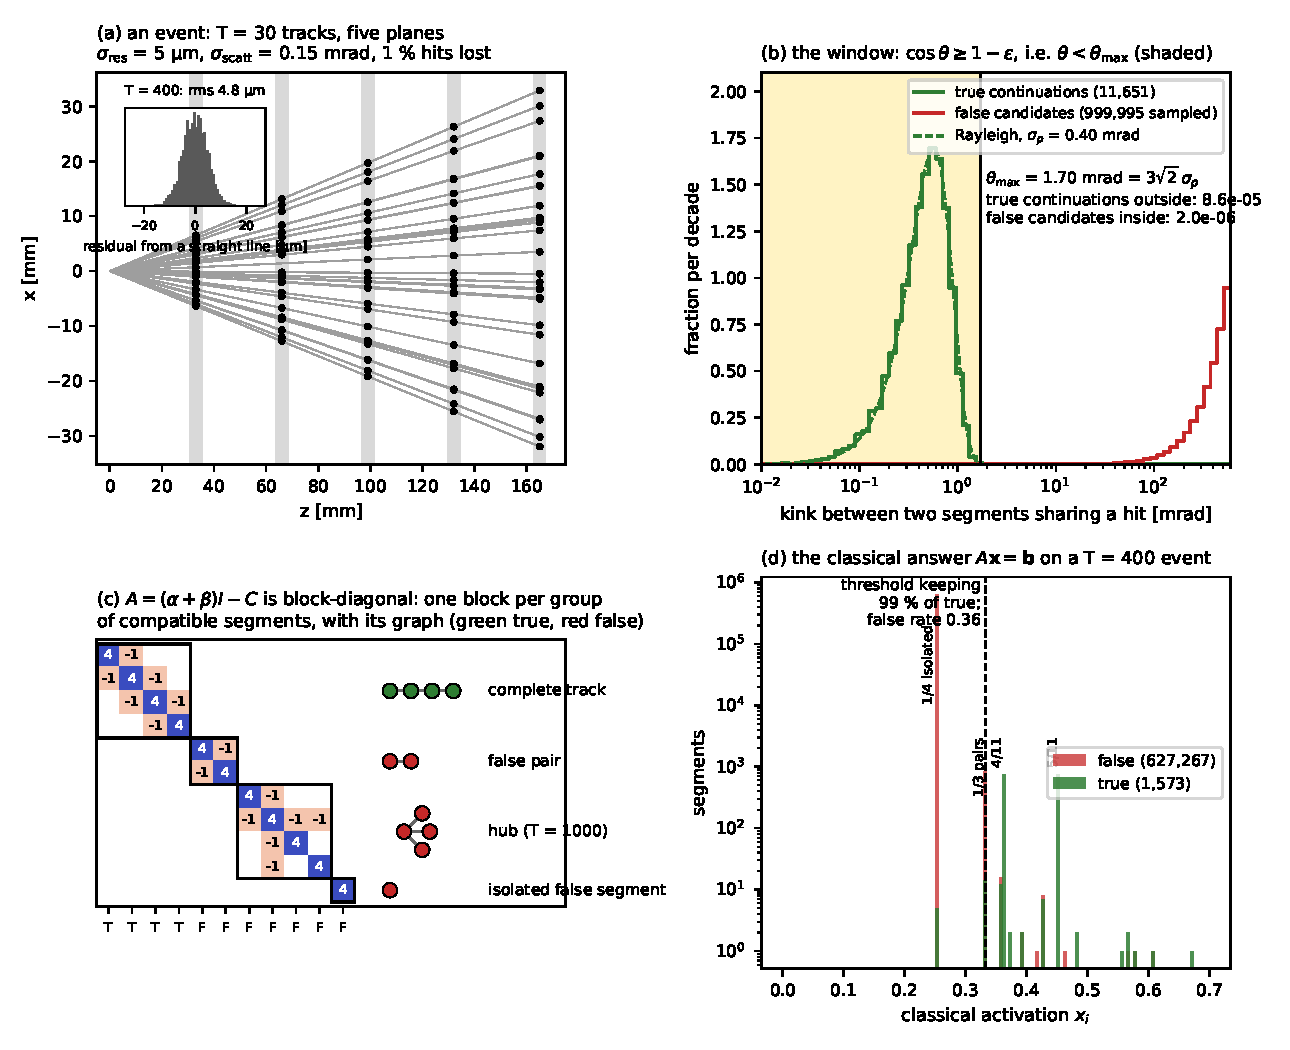
\includegraphics[width=0.98\textwidth]{fig1_hits_to_hamiltonian.pdf}
\caption{Figure 1. (a) An event and the hit residuals. (b) Kinks of true continuations (Rayleigh, $\sigma_p$) and of false candidates, with the window. (c) Real blocks of $A$ from a $T=400$ event. (d) Classical activations with the $99\%$ threshold. \src{corpus script 10\_fig\_hits\_to\_hamiltonian.py}}
\end{figure}

\subsection{The one-bit filter, and why it keeps what it keeps}
\msg{The filter multiplies each eigencomponent by $\cos(\lambda t/2)$; the zero sits on the isolated line; every other configuration keeps a factor fixed by its eigenvalues, and every hub keeps more of itself than a real track does.}
\begin{gather}
p_i=\Big[\cos^{2}\!\big(\tfrac{At}{2}\big)\mathbf{u}\Big]_i^{2}+\Big[\tfrac12\sin(At)\mathbf{u}\Big]_i^{2},\qquad t=\frac{\pi}{s},\\
|\cos(\lambda t/2)|:\ 0\ (\text{isolated}),\ 0.38\ (\text{pair}),\ 0.53\ (\text{triple}),\ 0.59\ (\text{track}),\ 0.63\ \text{and}\ 0.77\ (\text{hubs of 3 and 5 prongs}).
\end{gather}
\begin{figure}[H]\centering
\resizebox{0.98\textwidth}{!}{% Figure 2 of paper 1 (16 Sep 2026): the one-bit filter, and the QSVT with the dilation encoding.
% Built from circuits.tex panel (b) and circuits_qsvt.tex panel (a); requires circuit_styles.tex.
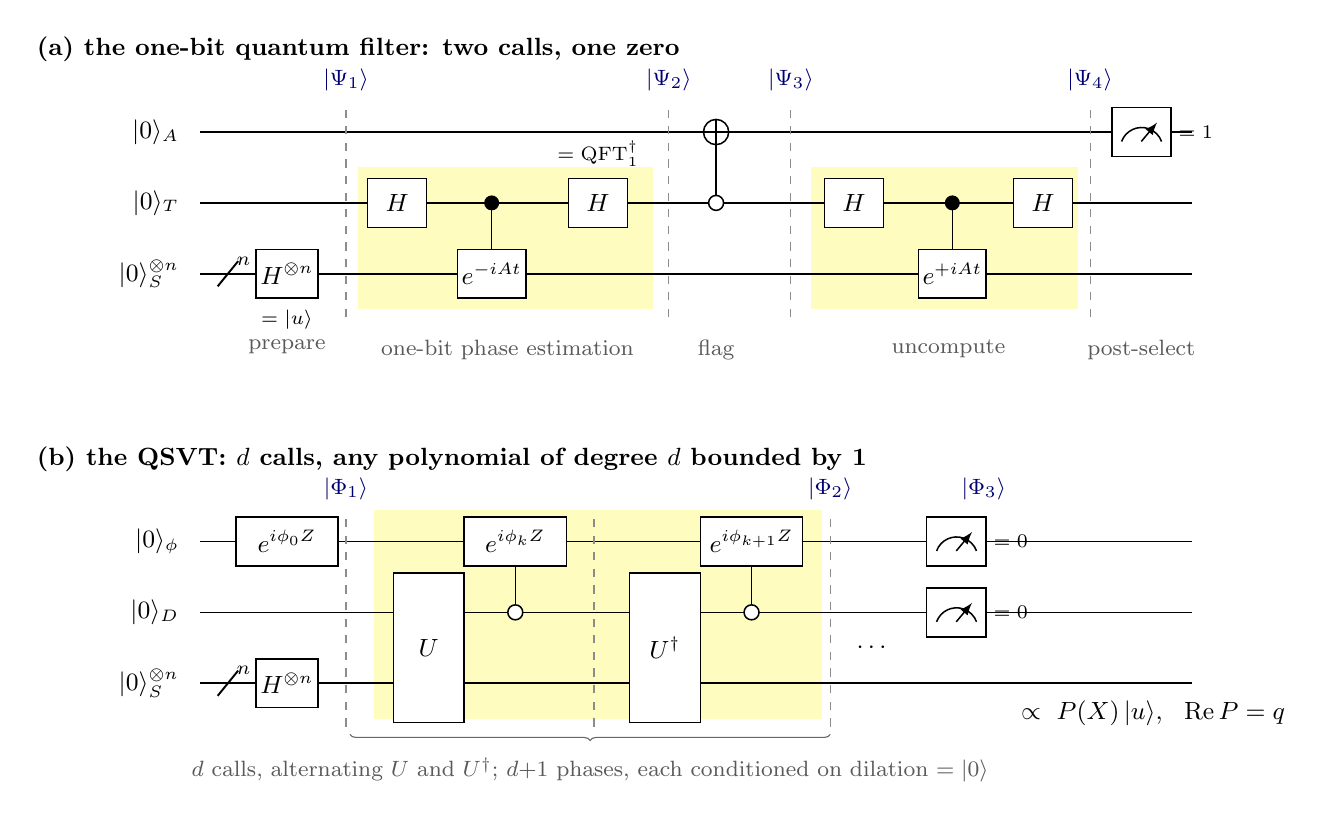
\begin{tikzpicture}[x=1cm,y=1cm]
\begin{scope}[shift={(0,0)}]
\fill[yellow!25] (2.0,-1.35) rectangle (5.75,0.45); \fill[yellow!25] (7.75,-1.35) rectangle (11.15,0.45);
\node[anchor=west,font=\small\bfseries] at (-2.2,1.95) {(a) the one-bit quantum filter: two calls, one zero};
\node[reg] at (-0.15,0.9)  {$|0\rangle_{A}$};
\node[reg] at (-0.15,0)    {$|0\rangle_{T}$};
\node[reg] at (-0.15,-0.9) {$|0\rangle^{\otimes n}_{S}$};
\draw[wire] (0,0.9) -- (12.6,0.9); \draw[wire] (0,0) -- (12.6,0); \draw[wire] (0,-0.9) -- (12.6,-0.9);
\slashwire{0.35}{-0.9}{$n$}
\node[gate] at (1.1,-0.9) {$H^{\otimes n}$};
\node[font=\scriptsize,anchor=north] at (1.1,-1.24) {$=|u\rangle$};
\vsep{1.85}{-1.45}{1.25}
\node[gate] at (2.5,0) {$H$};
\node[ctrl] at (3.7,0) {}; \draw[wire] (3.7,0) -- (3.7,-0.9); \node[gate] at (3.7,-0.9) {$e^{-iAt}$};
\node[gate] at (5.05,0) {$H$};
\node[font=\scriptsize,anchor=south] at (5.05,0.34) {$=\mathrm{QFT}_1^{\dagger}$};
\vsep{5.95}{-1.45}{1.25}
\node[octrl] at (6.55,0) {}; \draw[wire] (6.55,0.09) -- (6.55,0.9); \node[targ] at (6.55,0.9) {}; \draw[wire] (6.55,0.74) -- (6.55,1.06);
\vsep{7.5}{-1.45}{1.25}
\node[gate] at (8.3,0) {$H$};
\node[ctrl] at (9.55,0) {}; \draw[wire] (9.55,0) -- (9.55,-0.9); \node[gate] at (9.55,-0.9) {$e^{+iAt}$};
\node[gate] at (10.7,0) {$H$};
\vsep{11.3}{-1.45}{1.25}
\node[meter] at (11.95,0.9) {}; \draw[wire] (11.7,0.78) arc (160:20:0.27); \draw[wire,-latex] (11.95,0.78) -- (12.15,1.02);
\node[font=\scriptsize,anchor=west] at (12.3,0.9) {$=1$};
\node[blk] at (1.1,-1.62) {prepare};
\node[blk] at (3.9,-1.62) {one-bit phase estimation};
\node[blk] at (6.55,-1.62) {flag};
\node[blk] at (9.5,-1.62) {uncompute};
\node[blk] at (11.95,-1.62) {post-select};
\node[st] at (1.85,1.3) {$|\Psi_1\rangle$}; \node[st] at (5.95,1.3) {$|\Psi_2\rangle$};
\node[st] at (7.5,1.3) {$|\Psi_3\rangle$}; \node[st] at (11.3,1.3) {$|\Psi_4\rangle$};
\end{scope}
\begin{scope}[shift={(0,-5.2)}]
\fill[yellow!25] (2.2,-1.35) rectangle (7.9,1.3);
\node[anchor=west,font=\small\bfseries] at (-2.2,1.95) {(b) the QSVT: $d$ calls, any polynomial of degree $d$ bounded by 1};
\node[reg] at (-0.15,0.9)  {$|0\rangle_{\phi}$};
\node[reg] at (-0.15,0)    {$|0\rangle_{D}$};
\node[reg] at (-0.15,-0.9) {$|0\rangle^{\otimes n}_{S}$};
\draw[wire] (0,0.9) -- (12.6,0.9); \draw[wire] (0,0) -- (12.6,0); \draw[wire] (0,-0.9) -- (12.6,-0.9);
\slashwire{0.35}{-0.9}{$n$}
\node[gate] at (1.1,-0.9) {$H^{\otimes n}$};
\node[gate,minimum width=13mm] at (1.1,0.9) {$e^{i\phi_0 Z}$};
\vsep{1.85}{-1.45}{1.25}
% one repetition: U on (D,S), then the projector-controlled phase on the signal qubit
\node[gate,minimum height=19mm,minimum width=9mm] at (2.9,-0.45) {$U$};
\node[octrl] at (4.0,0) {}; \draw[wire] (4.0,0.09) -- (4.0,0.62);
\node[gate,minimum width=13mm] at (4.0,0.9) {$e^{i\phi_k Z}$};
\vsep{5.0}{-1.45}{1.25}
\node[gate,minimum height=19mm,minimum width=9mm] at (5.9,-0.45) {$U^{\dagger}$};
\node[octrl] at (7.0,0) {}; \draw[wire] (7.0,0.09) -- (7.0,0.62);
\node[gate,minimum width=13mm] at (7.0,0.9) {$e^{i\phi_{k+1} Z}$};
\vsep{8.0}{-1.45}{1.25}
\node[font=\small] at (8.55,-0.45) {$\cdots$};
\draw[brace] (1.9,-1.55) -- (8.0,-1.55); \node[blk] at (4.95,-1.72) {$d$ calls, alternating $U$ and $U^{\dagger}$; $d{+}1$ phases, each conditioned on dilation $=|0\rangle$};
\node[meter] at (9.6,0.9) {}; \draw[wire] (9.35,0.78) arc (160:20:0.27); \draw[wire,-latex] (9.6,0.78) -- (9.8,1.02);
\node[font=\scriptsize,anchor=west] at (9.95,0.9) {$=0$};
\node[meter] at (9.6,0) {}; \draw[wire] (9.35,-0.12) arc (160:20:0.27); \draw[wire,-latex] (9.6,-0.12) -- (9.8,0.12);
\node[font=\scriptsize,anchor=west] at (9.95,0) {$=0$};
\node[font=\small,anchor=north west] at (10.3,-1.0) {$\propto\ P(X)\,|u\rangle,\ \ \mathrm{Re}\,P=q$};
\node[st] at (1.85,1.3) {$|\Phi_1\rangle$}; \node[st] at (8.0,1.3) {$|\Phi_2\rangle$}; \node[st] at (9.95,1.3) {$|\Phi_3\rangle$};
\end{scope}
\end{tikzpicture}
}
\caption{Figure 2. (a) The one-bit filter, correctly wired. (b) The QSVT with the dilation encoding. The difference is boxed. \src{hand-drawn TikZ}}
\end{figure}
\begin{figure}[H]\centering
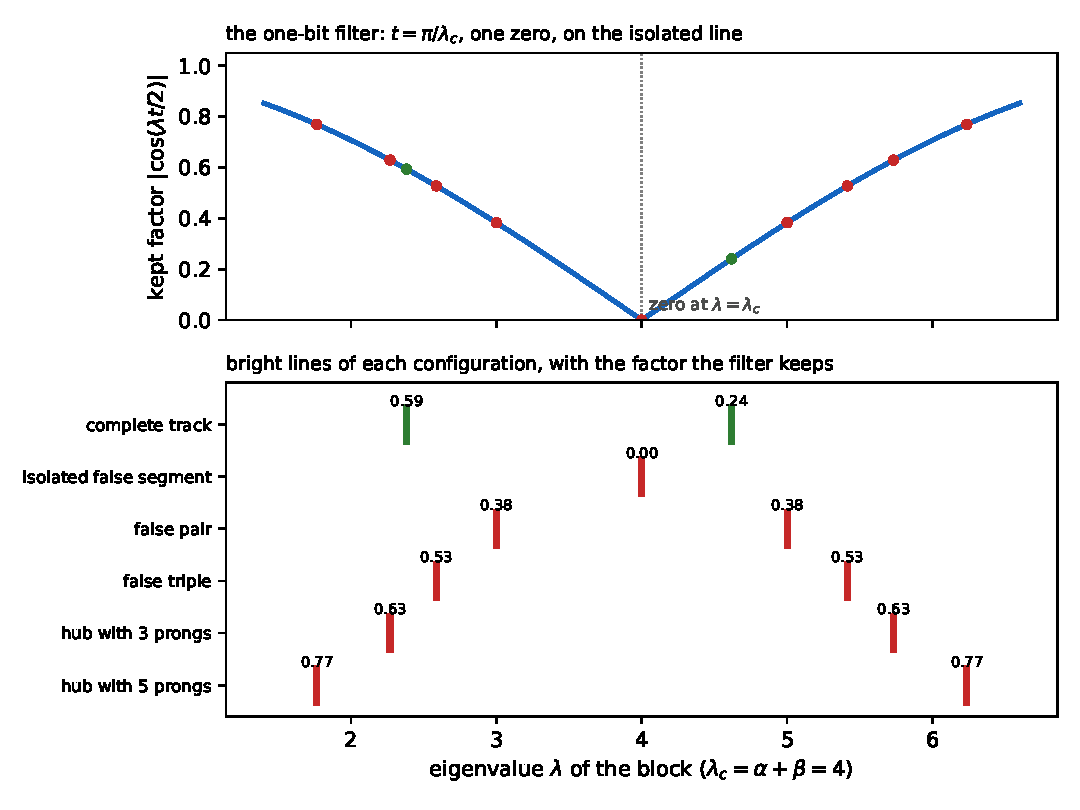
\includegraphics[width=0.7\textwidth]{fig2_onebit_response.pdf}
\caption{Figure 2 (companion). The kept factor on each configuration's bright lines. \src{corpus script 11\_fig\_onebit\_response.py}}
\end{figure}

\subsection{What each solver keeps}
\msg{Noise creates seven error types. At $99\%$ efficiency the classical solver and the one-bit filter keep every false pair; the QSVT keeps every complete track and removes every false pair; its lost efficiency is broken and contaminated tracks only.}
\begin{figure}[H]\centering
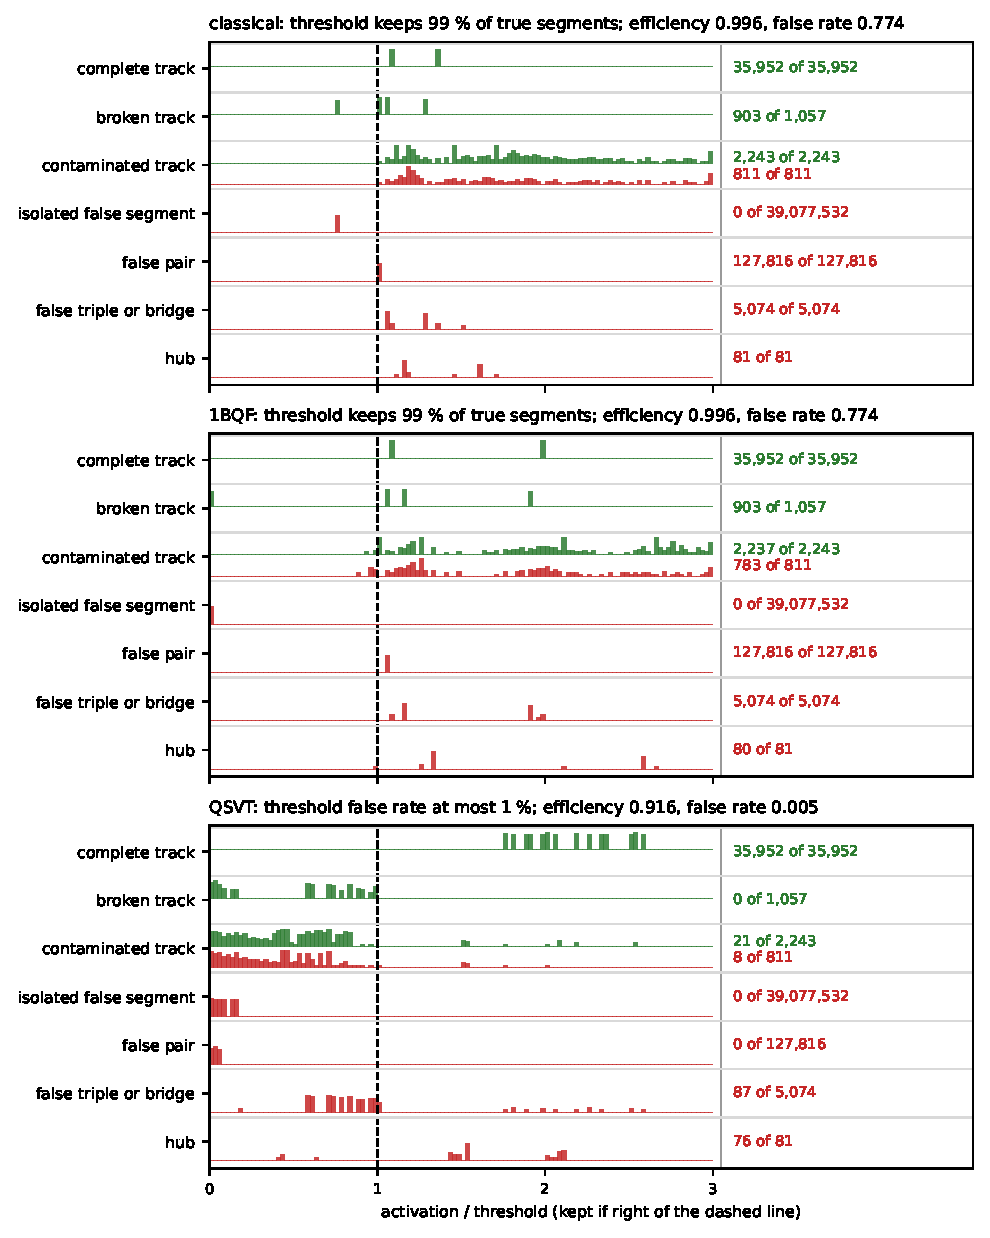
\includegraphics[width=0.98\textwidth]{fig3_error_atlas_T1000_with_qsvt.pdf}
\caption{Figure 3. Activation by error type at $T=1000$, ten events pooled, with each solver's threshold; counts of kept segments at the right of each row. Companion at $T=400$ in the supplement. \src{corpus script 12\_fig\_error\_atlas.py}}
\end{figure}
\begin{center}\footnotesize
\begin{tabular}{lcccc}\toprule
 & $T=200$ & $T=400$ & $T=700$ & $T=1000$\\\midrule
classical: false rate at $99\%$ efficiency & $0.12$ & $0.35$ & $0.63$ & $0.77$\\
one-bit filter: false rate at $99\%$ efficiency & $0.12$ & $0.35$ & $0.63$ & $0.77$\\
QSVT: efficiency at false rate $\le1\%$ & $0.984$ & $0.973$ & $0.937$ & $0.917$\\
QSVT: lowest efficiency over the ten events & $0.969$ & $0.938$ & $0.919$ & $0.893$\\\bottomrule
\end{tabular}\\[2pt]
\src{medians over ten events; corpus outputs\_5um/summary\_by\_event.csv}
\end{center}
\noindent At $T=1000$ (ten events): the classical solver and the one-bit filter keep all $127{,}816$ false-pair segments and all $5{,}074$ false-triple segments; the QSVT keeps $0$ false-pair segments, keeps all $35{,}952$ segments of complete tracks, and loses $1{,}057$ broken-track and $2{,}222$ contaminated-track true segments.

\subsection{The one change}
\msg{Every error type sits on known eigenvalues, so the fix is not a new primitive but more zeros: $d$ calls, any bounded polynomial of degree $d$ (Figure 2b). Results 2 shows where the lines lie; Results 3 which polynomial to apply.}

\subsection*{Notes for George (not paper text)}
\begin{itemize}[leftmargin=1.5em,itemsep=1pt]
\item On most events the one-bit filter and the classical solver read the same false rate at $99\%$: both thresholds land on the $1/3$ level shared by broken tracks and false pairs. The message is ``the one-bit filter keeps a high false rate'', not ``worse than classical''.
\item Read at the same false rate as the QSVT ($\le1\%$), the classical solver keeps $97.5\%$ at $T=400$ on the median event but only $49\%$ at $T=700$ and $24\%$ at $T=1000$; the one-bit filter keeps $49\%$ at all three. The like-for-like advantage is decisive from $T=700$.
\item At $T=20$ and $50$ the $99\%$ reading is volatile (false rate $0$ to $0.98$ between events): a single broken track sits on the isolated level. Plot medians with the event range.
\item The figures were built and every number checked in code; the image viewer was unavailable in this session, so they have not been inspected by eye.
\end{itemize}

\section{The problem as a spectrum}
\msg{Geometry pins every true track to the same five-hit chain, whose four eigenvalues are known in closed form; every false configuration is a small graph with known lines.}
\begin{gather}
\lambda(A)=s-\lambda(C),\qquad
\lambda_{\rm true}\in\{s-2\cos(k\pi/5)\}_{k=1}^{4}=\{2.382,\,3.382,\,4.618,\,5.618\},\\
x_{\rm outer}(m)=\tfrac12-\frac{r+r^{m}}{2(1+r^{m+1})},\qquad r=2-\sqrt3 .\qquad\text{[ch.~2.4, 2.7]}
\end{gather}
\begin{gather}
\text{isolated: }\lambda=s;\qquad\text{pair }P_2:\ s\mp1;\qquad\text{triple }P_3:\ \{s,\,s\mp\sqrt2\};\\
\text{hub }K_{1,m}:\ s\pm\sqrt m\ \text{ plus }m{-}1\text{ copies of }s.\qquad\text{[ch.~2.7]}
\end{gather}
\begin{equation}
\varepsilon=\sqrt{\,2(\kappa\sigma_{\rm scatt})^{2}+12\arctan^{2}\!\big(\kappa\sigma_{\rm res}/\Delta z\big)+2\theta_{\min}^{2}\,},\qquad \kappa=3,\ \Delta z=33\,\text{mm},\ \theta_{\min}=15\,\mu\text{rad}.\quad\text{[ch.~2.2]}
\end{equation}
\begin{figure}[H]\centering
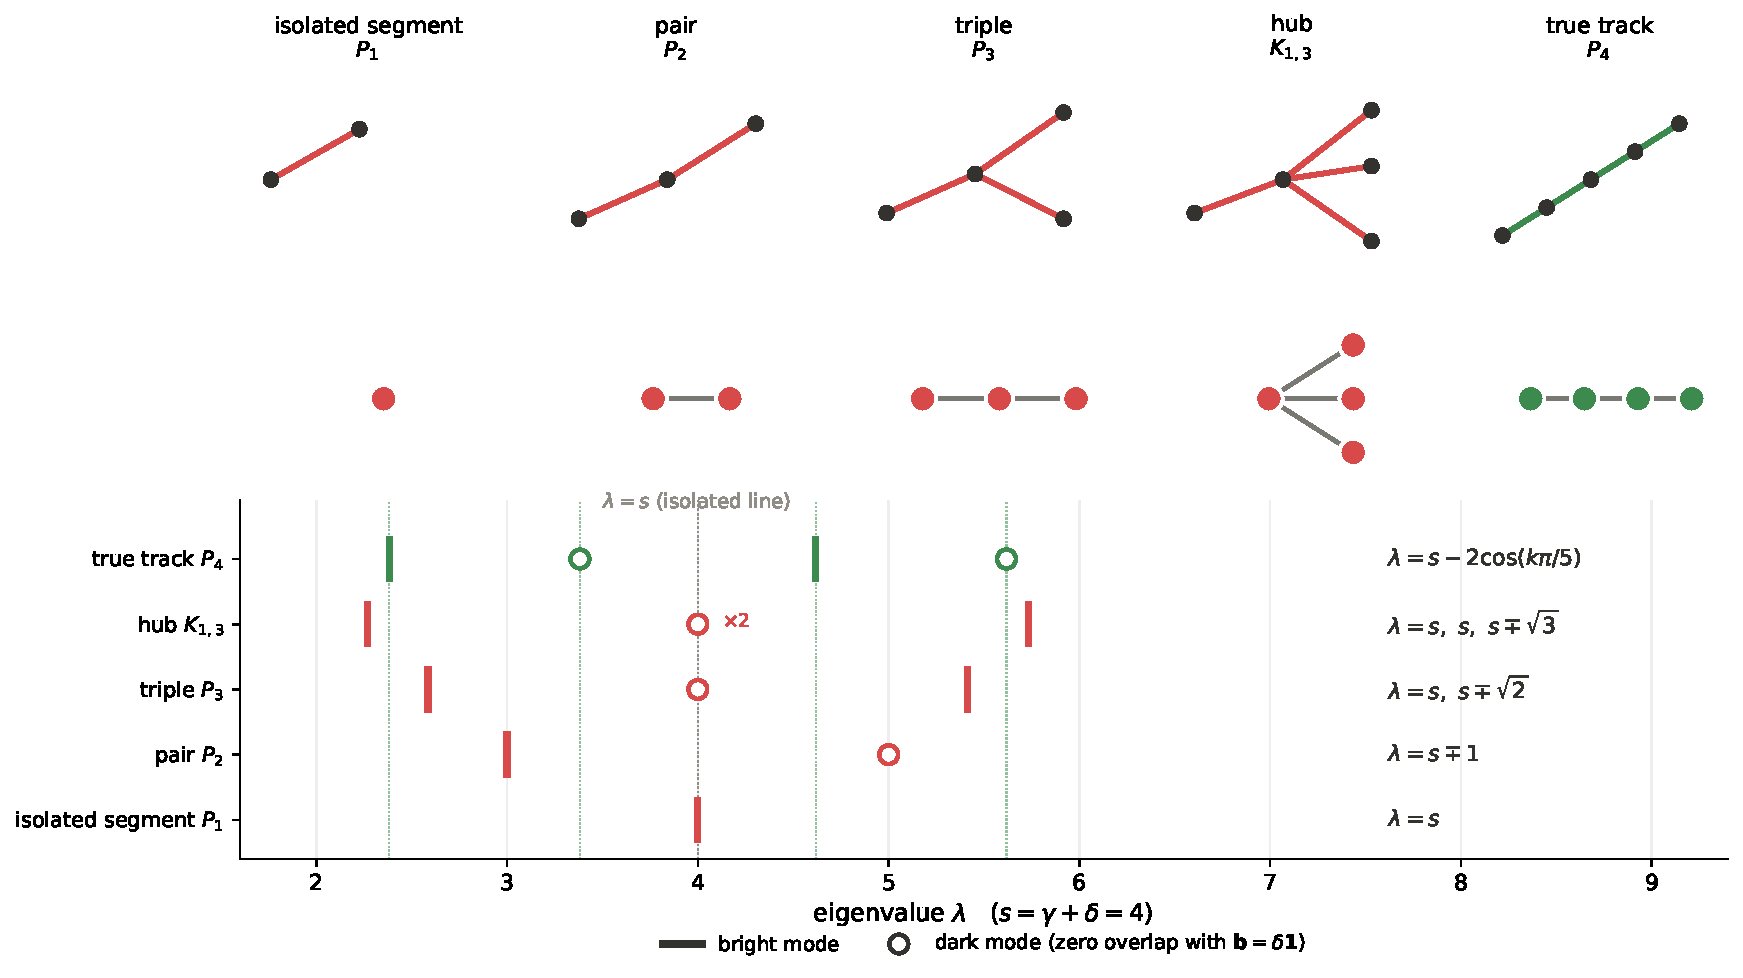
\includegraphics[width=0.98\textwidth]{motif_gallery.pdf}
\caption{Figure 2. The motif gallery: each cluster type with its eigenvalue lines against the four true lines. \src{fig\_motifs, ch.~2.3}}
\end{figure}
\begin{figure}[H]\centering
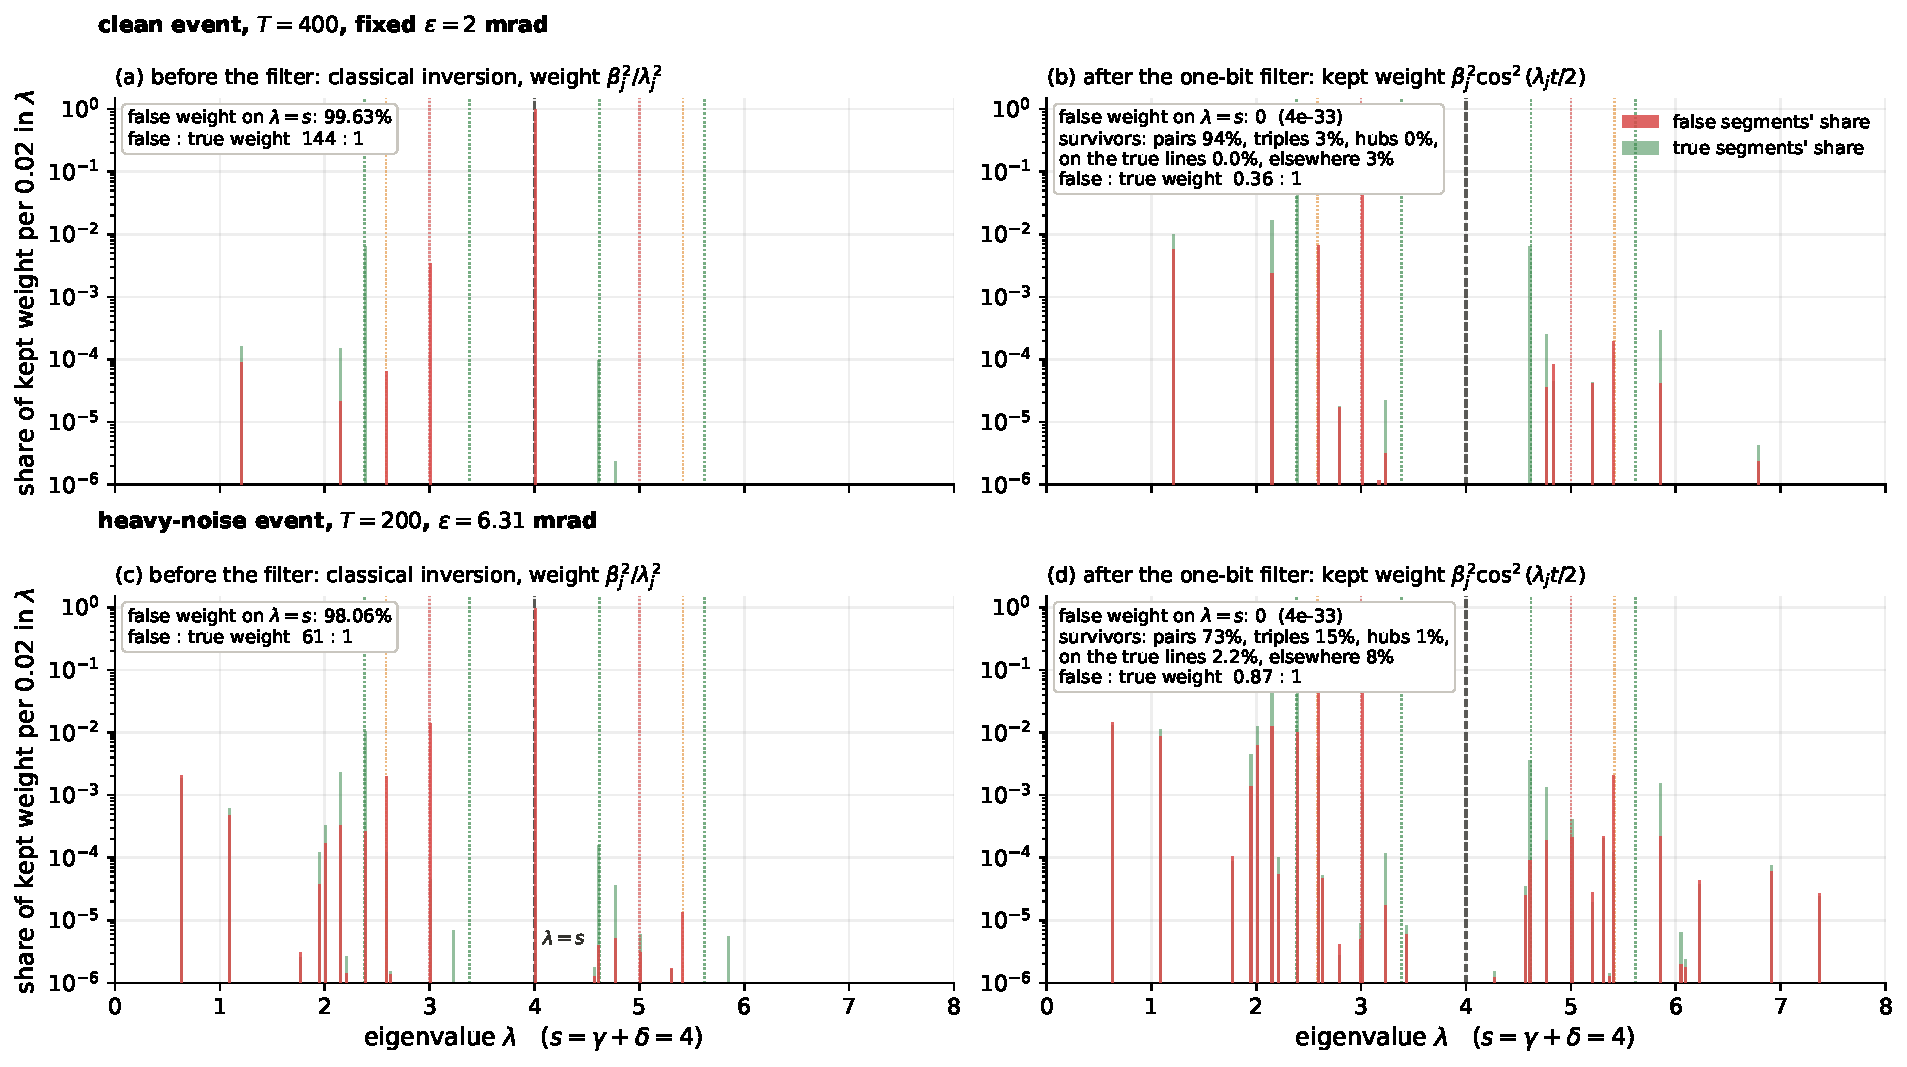
\includegraphics[width=0.85\textwidth]{notch_spectrum.pdf}
\caption{Figure 2 (companion, may go to the supplement). The single zero on the spectrum and where the surviving false segments live. \src{fig\_notch\_spectrum, ch.~3.2}}
\end{figure}
\noindent Numbers: census on clean $T=200$ events, median true--false gap $0.228$, none strictly degenerate with a true chain [ch.~2.7].

\section{The QSVT on this primitive}
\msg{A quantum computer applies any bounded polynomial of $A$ at a cost linear in its degree; the 1BQF is the degree-one member; the comb puts narrow inverse passes on the four true lines and nothing else.}
\begin{gather}
(\langle0|\otimes I)\,U\,(|0\rangle\otimes I)=X,\qquad
U_{\Phi}=e^{i\phi_0(2\Pi-I)}\prod_{k=1}^{d}\Big[U^{(\dagger)}e^{i\phi_k(2\Pi-I)}\Big],\\
\big\langle0\big|W^{k}\big|0\big\rangle_{\rm dil}=T_k(X),\qquad
p(X)=\sum_{k=0}^{d}c_k\,T_k(X),\qquad
P_{\rm anc}=\frac{\lVert p(X)|u\rangle\rVert^{2}}{(\sum_k|c_k|)^{2}},\\
d\ \approx\ \frac{2W}{h}\quad\text{(a feature of width $h$ on a spectral span $W$)}.\qquad\text{[ch.~4.1 to 4.3]}
\end{gather}
\begin{figure}[H]\centering
\resizebox{0.98\textwidth}{!}{% Two further realisations of the same polynomial response (section 4.2), to
% the conventions of figure~\ref{fig:circuits}: (a) the phase sequence, the
% literature's QSVT; (b) the trigonometric comb over the one-bit filter's own
% evolution (QETU).  The LCU realisation is figure~\ref{fig:circuits}(c).
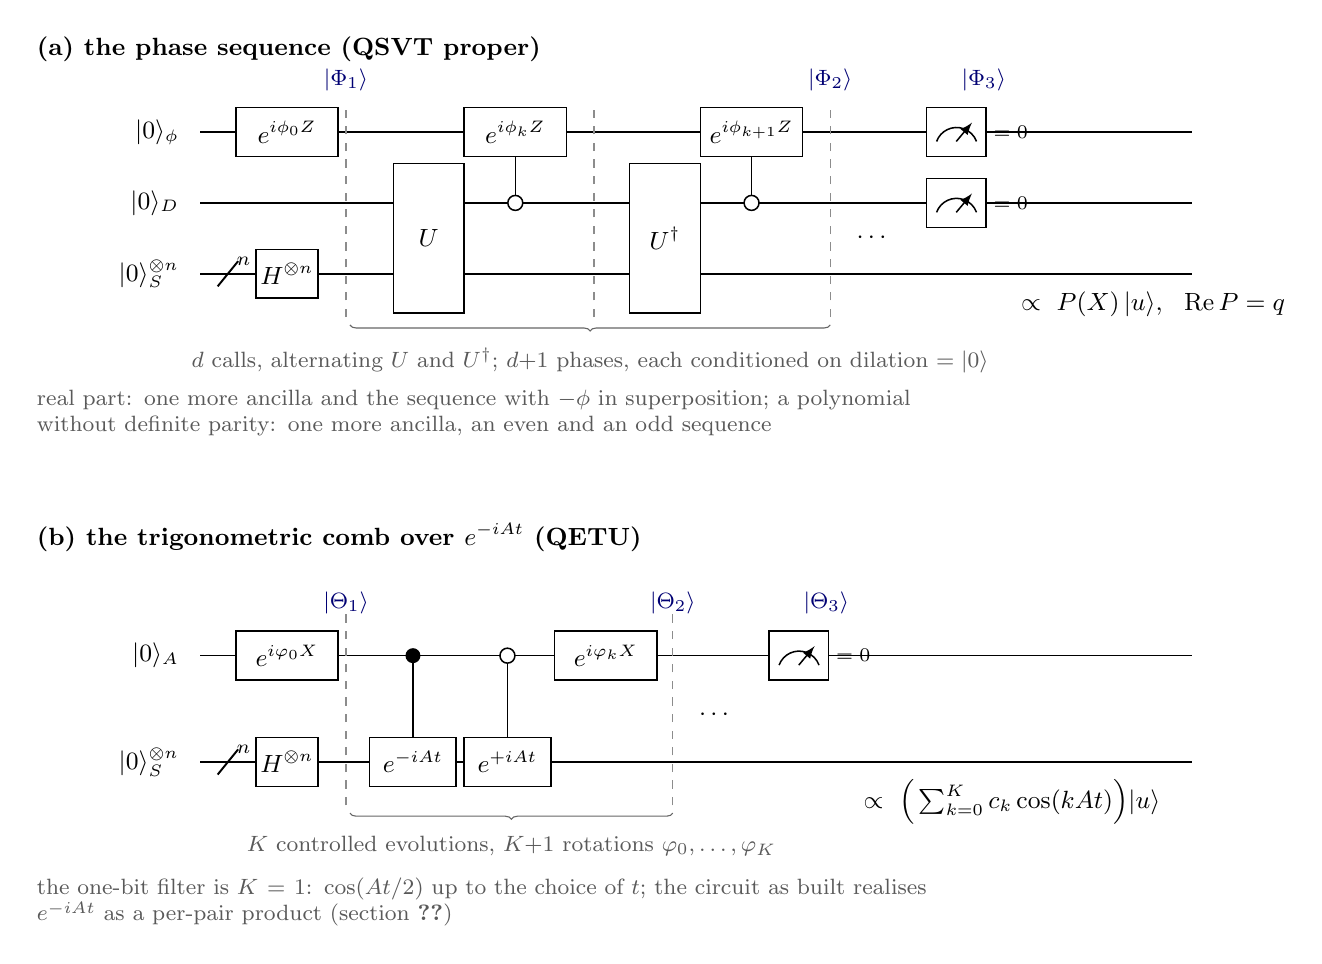
\begin{tikzpicture}[x=1cm,y=1cm]
% ─────────────── (a) the phase sequence ───────────────
\begin{scope}[shift={(0,0)}]
\node[anchor=west,font=\small\bfseries] at (-2.2,1.95) {(a) the phase sequence (QSVT proper)};
\node[reg] at (-0.15,0.9)  {$|0\rangle_{\phi}$};
\node[reg] at (-0.15,0)    {$|0\rangle_{D}$};
\node[reg] at (-0.15,-0.9) {$|0\rangle^{\otimes n}_{S}$};
\draw[wire] (0,0.9) -- (12.6,0.9); \draw[wire] (0,0) -- (12.6,0); \draw[wire] (0,-0.9) -- (12.6,-0.9);
\slashwire{0.35}{-0.9}{$n$}
\node[gate] at (1.1,-0.9) {$H^{\otimes n}$};
\node[gate,minimum width=13mm] at (1.1,0.9) {$e^{i\phi_0 Z}$};
\vsep{1.85}{-1.45}{1.25}
% one repetition: U on (D,S), then the projector-controlled phase on the signal qubit
\node[gate,minimum height=19mm,minimum width=9mm] at (2.9,-0.45) {$U$};
\node[octrl] at (4.0,0) {}; \draw[wire] (4.0,0.09) -- (4.0,0.62);
\node[gate,minimum width=13mm] at (4.0,0.9) {$e^{i\phi_k Z}$};
\vsep{5.0}{-1.45}{1.25}
\node[gate,minimum height=19mm,minimum width=9mm] at (5.9,-0.45) {$U^{\dagger}$};
\node[octrl] at (7.0,0) {}; \draw[wire] (7.0,0.09) -- (7.0,0.62);
\node[gate,minimum width=13mm] at (7.0,0.9) {$e^{i\phi_{k+1} Z}$};
\vsep{8.0}{-1.45}{1.25}
\node[font=\small] at (8.55,-0.45) {$\cdots$};
\draw[brace] (1.9,-1.55) -- (8.0,-1.55); \node[blk] at (4.95,-1.72) {$d$ calls, alternating $U$ and $U^{\dagger}$; $d{+}1$ phases, each conditioned on dilation $=|0\rangle$};
\node[meter] at (9.6,0.9) {}; \draw[wire] (9.35,0.78) arc (160:20:0.27); \draw[wire,-latex] (9.6,0.78) -- (9.8,1.02);
\node[font=\scriptsize,anchor=west] at (9.95,0.9) {$=0$};
\node[meter] at (9.6,0) {}; \draw[wire] (9.35,-0.12) arc (160:20:0.27); \draw[wire,-latex] (9.6,-0.12) -- (9.8,0.12);
\node[font=\scriptsize,anchor=west] at (9.95,0) {$=0$};
\node[font=\small,anchor=north west] at (10.3,-1.0) {$\propto\ P(X)\,|u\rangle,\ \ \mathrm{Re}\,P=q$};
\node[st] at (1.85,1.3) {$|\Phi_1\rangle$}; \node[st] at (8.0,1.3) {$|\Phi_2\rangle$}; \node[st] at (9.95,1.3) {$|\Phi_3\rangle$};
\node[anchor=north west,font=\footnotesize,text=black!65,text width=11.5cm,align=left] at (-2.2,-2.25) {real part: one more ancilla and the sequence with $-\phi$ in superposition; a polynomial without definite parity: one more ancilla, an even and an odd sequence};
\end{scope}
% ─────────────── (b) the trigonometric comb over e^{-iAt} ───────────────
\begin{scope}[shift={(0,-6.2)}]
\node[anchor=west,font=\small\bfseries] at (-2.2,1.95) {(b) the trigonometric comb over $e^{-iAt}$ (QETU)};
\node[reg] at (-0.15,0.45)  {$|0\rangle_{A}$};
\node[reg] at (-0.15,-0.9) {$|0\rangle^{\otimes n}_{S}$};
\draw[wire] (0,0.45) -- (12.6,0.45); \draw[wire] (0,-0.9) -- (12.6,-0.9);
\slashwire{0.35}{-0.9}{$n$}
\node[gate] at (1.1,-0.9) {$H^{\otimes n}$};
\node[gate,minimum width=13mm] at (1.1,0.45) {$e^{i\varphi_0 X}$};
\vsep{1.85}{-1.45}{1.0}
\node[ctrl] at (2.7,0.45) {}; \draw[wire] (2.7,0.45) -- (2.7,-0.9); \node[gate,minimum width=11mm] at (2.7,-0.9) {$e^{-iAt}$};
\node[octrl] at (3.9,0.45) {}; \draw[wire] (3.9,0.36) -- (3.9,-0.9); \node[gate,minimum width=11mm] at (3.9,-0.9) {$e^{+iAt}$};
\node[gate,minimum width=13mm] at (5.15,0.45) {$e^{i\varphi_k X}$};
\vsep{6.0}{-1.45}{1.0}
\node[font=\small] at (6.55,-0.3) {$\cdots$};
\draw[brace] (1.9,-1.55) -- (6.0,-1.55); \node[blk] at (3.95,-1.72) {$K$ controlled evolutions, $K{+}1$ rotations $\varphi_0,\dots,\varphi_K$};
\node[meter] at (7.6,0.45) {}; \draw[wire] (7.35,0.33) arc (160:20:0.27); \draw[wire,-latex] (7.6,0.33) -- (7.8,0.57);
\node[font=\scriptsize,anchor=west] at (7.95,0.45) {$=0$};
\node[font=\small,anchor=north west] at (8.3,-1.0) {$\propto\ \Big(\sum_{k=0}^{K} c_k\cos(kAt)\Big)|u\rangle$};
\node[st] at (1.85,0.85) {$|\Theta_1\rangle$}; \node[st] at (6.0,0.85) {$|\Theta_2\rangle$}; \node[st] at (7.95,0.85) {$|\Theta_3\rangle$};
\node[anchor=north west,font=\footnotesize,text=black!65,text width=11.5cm,align=left] at (-2.2,-2.25) {the one-bit filter is $K=1$: $\cos(At/2)$ up to the choice of $t$; the circuit as built realises $e^{-iAt}$ as a per-pair product (section~\ref{sec:fork:trotter})};
\end{scope}
\end{tikzpicture}
}
\caption{Figure 3 (candidate). The three realisations of the polynomial: the linear combination of walk powers, the phase sequence, the trigonometric comb over $e^{-iAt}$. \src{hand-drawn TikZ, ch.~4.2}}
\end{figure}
\begin{figure}[H]\centering
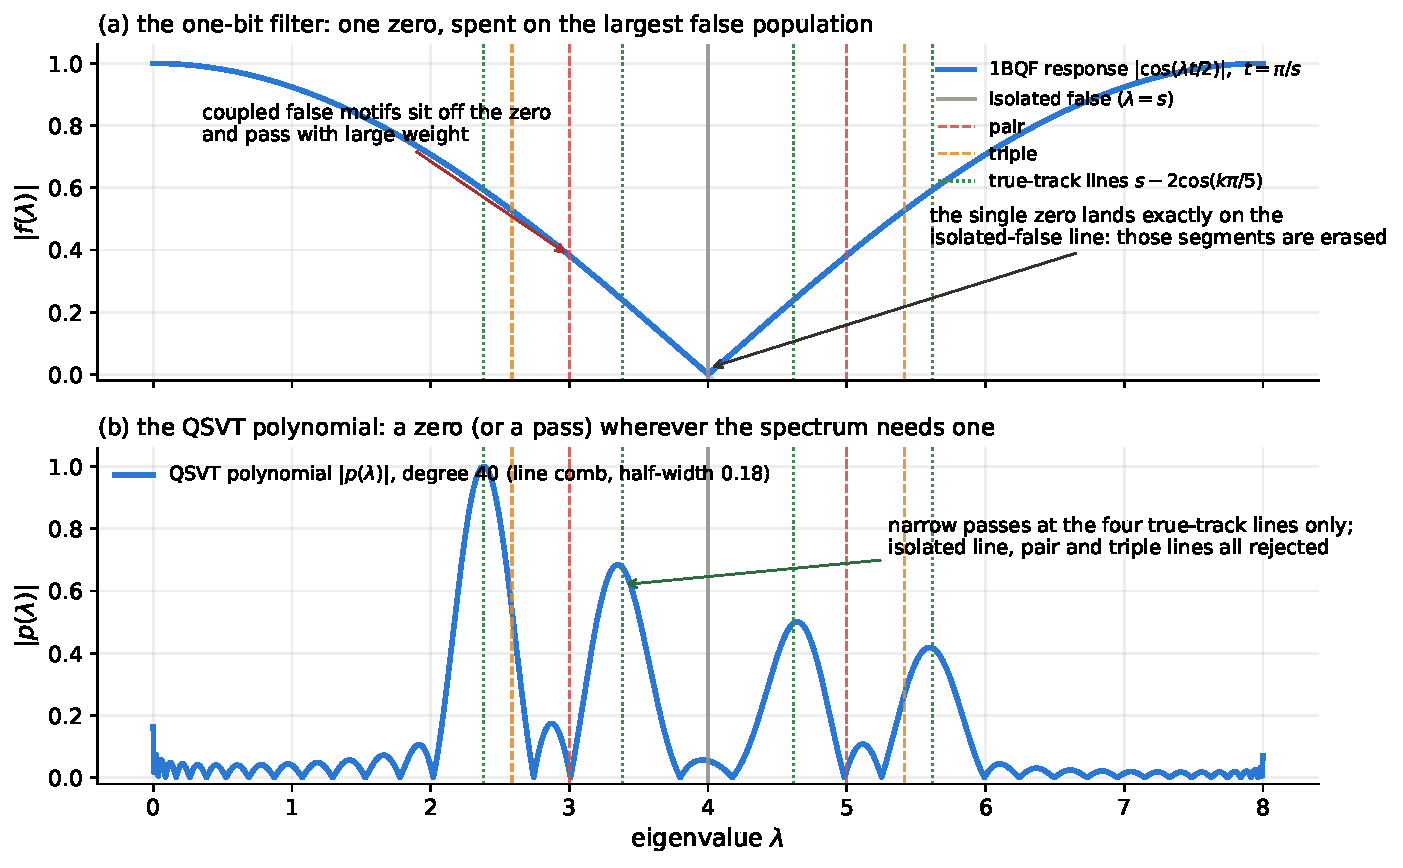
\includegraphics[width=0.58\textwidth]{response_functions.pdf}\hfill
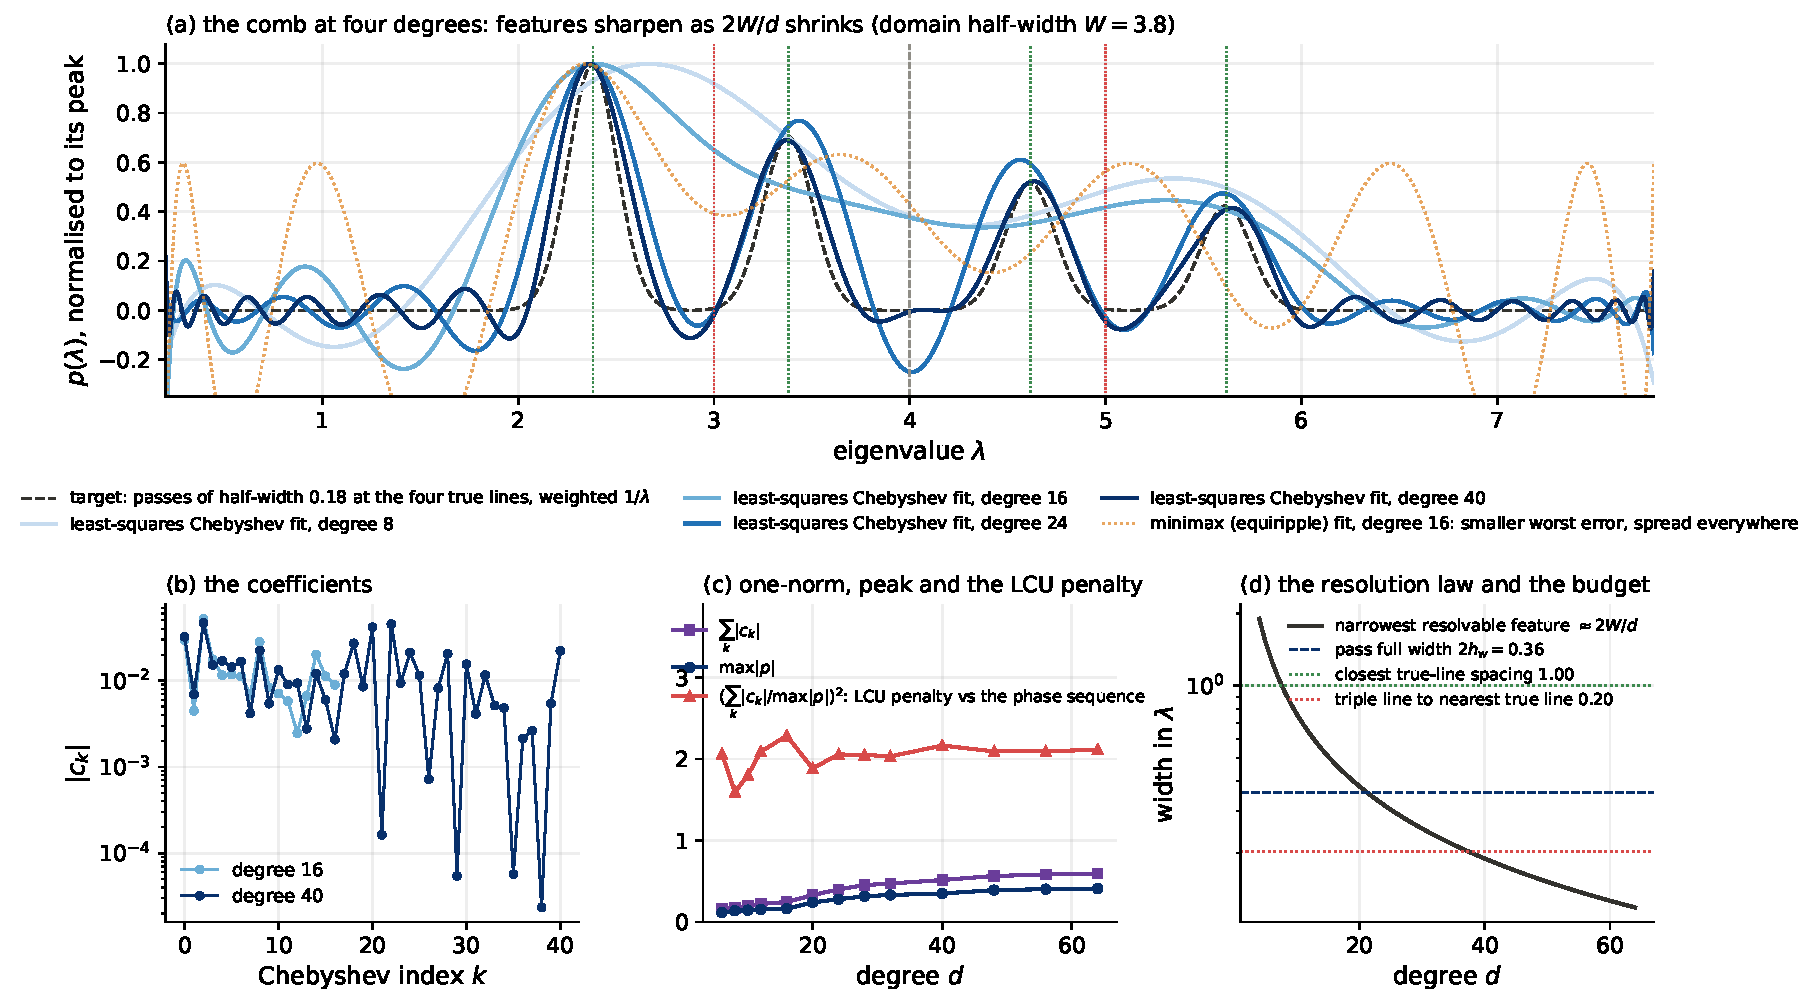
\includegraphics[width=0.40\textwidth]{comb_degrees.pdf}
\caption{Figure 3. Response functions on the spectrum (the one-bit cosine, the band-limited inverse, the line comb) and the degree ladder. \src{fig\_responses, fig\_comb\_degrees, ch.~4.3}}
\end{figure}
\noindent Numbers: production comb degree $40$, half-width $0.18$; metric-validated degree $12$--$20$ at $T=200$ [ch.~5.1, 10.1]. The band-limited inverse, the obvious first design, reads a $43.6\%$ false rate at $T=400$ [ch.~5.1].

\section{Results on clean events}
\msg{Every solver read at the threshold that keeps 99\,\% of its own true segments; the comb wins through 300 tracks and ties at 400 at the wide 2\,mrad acceptance; at the formula acceptance 1000 tracks are solved outright; the limit of every spectral filter is a graph-isomorphism degeneracy.}
\begin{gather}
\eff=\frac{n_{\rm true\,active}}{n_{\rm true}},\qquad
\far=\frac{n_{\rm false\,active}}{n_{\rm active}},\qquad
\tau:\ \text{lowest threshold with }\eff\ge0.99 .\qquad\text{[ch.~2.6]}\\
f(PAP^{\!\top})\,\mathbf{b}=P\,f(A)\,\mathbf{b}\quad\text{for every }f\text{ and every permutation }P\text{ with }P\mathbf{b}=\mathbf{b} .\qquad\text{[ch.~5.5]}
\end{gather}
\noindent The first line is the efficiency-first working point; the second says isomorphic components are twins under every spectral filter, classical scoring included.
\begin{figure}[H]\centering
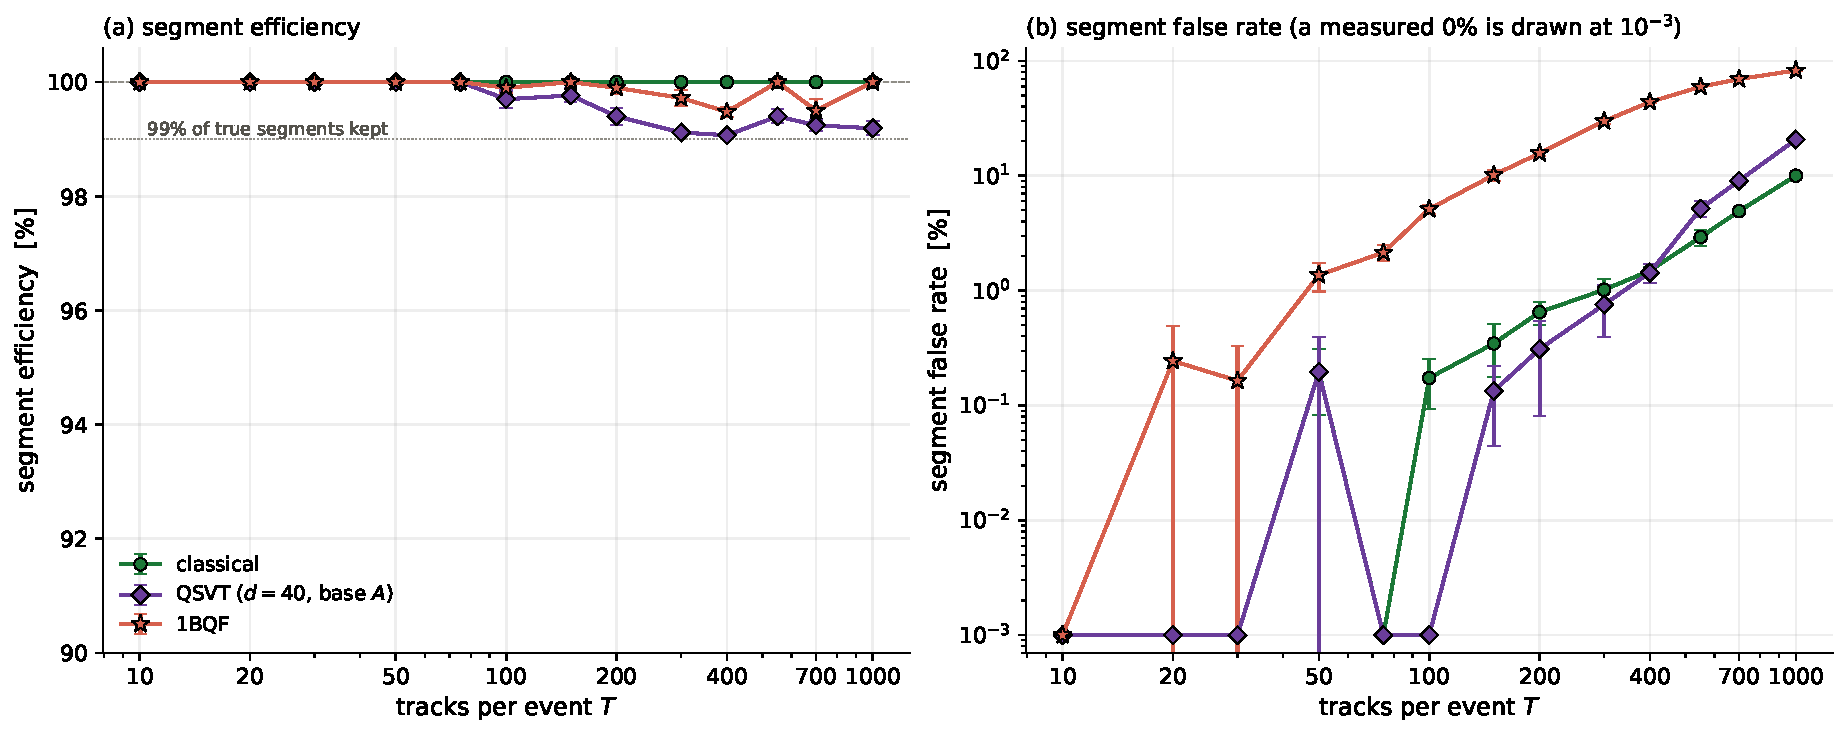
\includegraphics[width=0.95\textwidth]{clean_headline.pdf}
\caption{Figure 4. Segment efficiency (a) and false rate (b) against track count for the classical solver, the QSVT (degree 40, base Hamiltonian) and the 1BQF, each at its efficiency-first working point; $\gamma=3$, 2\,mrad, no hit drop. \src{fig\_clean2x2, ch.~5.2; the 1BQF curve is the stored package circuit}}
\end{figure}
\begin{figure}[H]\centering
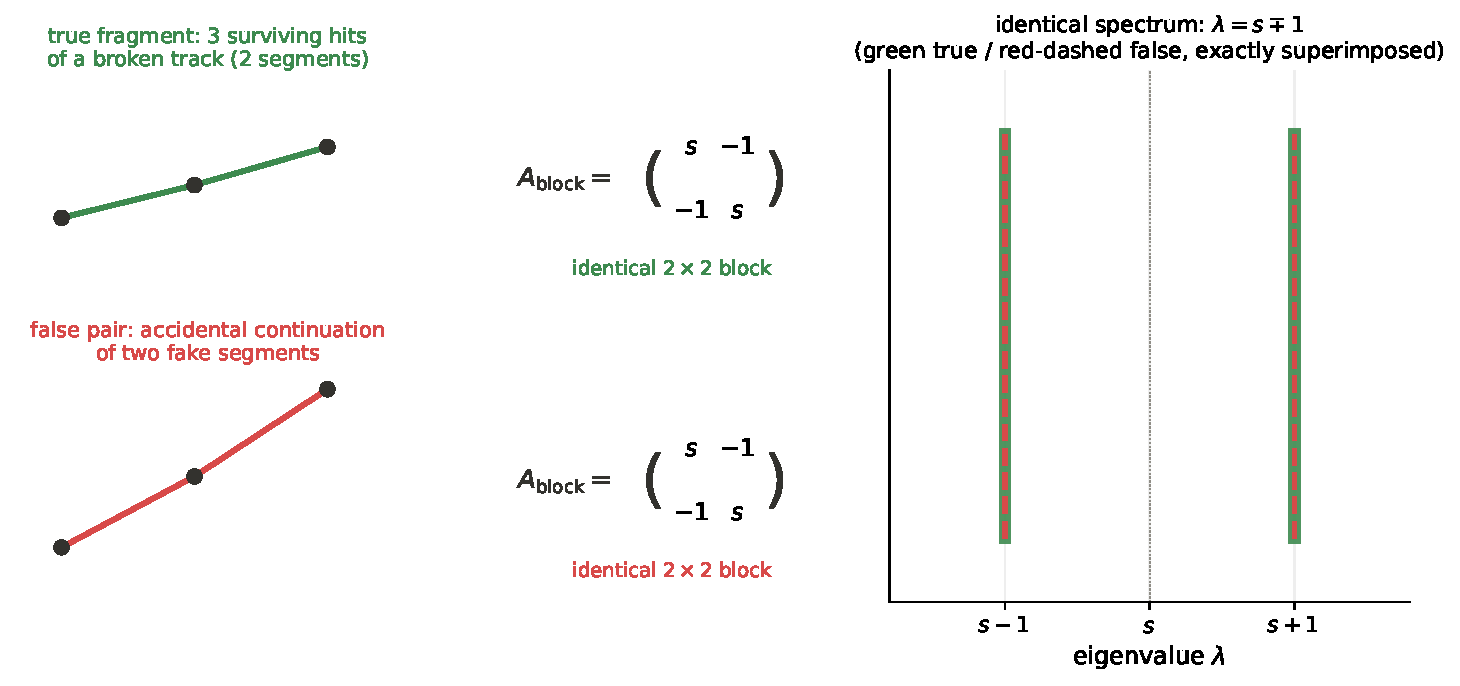
\includegraphics[width=0.55\textwidth]{spectral_twins.pdf}\hfill
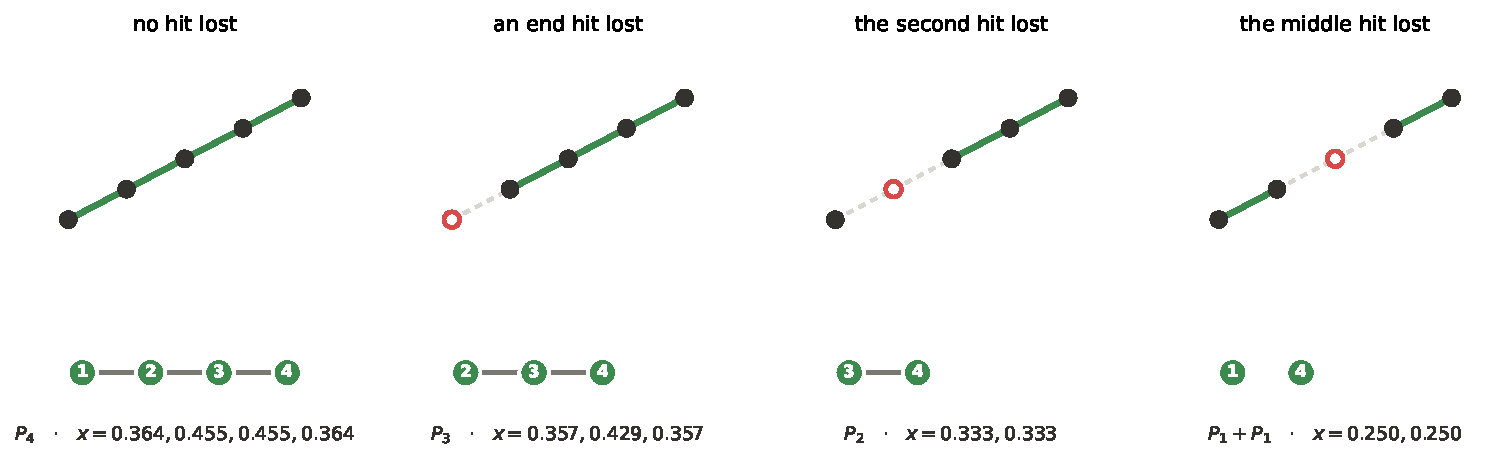
\includegraphics[width=0.42\textwidth]{fragmentation.pdf}
\caption{Figure 4 (companions, one paragraph each). Spectral twins; hit inefficiency makes fragments that sit off the comb lines. \src{fig\_twin, fig\_fragmentation, ch.~5.5, 5.3}}
\end{figure}
\begin{center}\footnotesize
\begin{tabular}{lccc}\toprule
False rate at the working point & $T=200$ & $T=400$ & $T=1000$, formula acceptance \\\midrule
Classical & $0.65\%$ & $1.49\%$ & --- \\
QSVT, degree 40, base $A$ & $0.31\%$ & $1.44\%$ & $0\%$ measured at $\eff=99.85\%$ \\
1BQF (package circuit) & --- & $43.9\%$ (at $\eff=99.5\%$) & --- \\\bottomrule
\end{tabular}\\[2pt]
\src{ch.~5.2, 10.4; every number at the working point defined above}
\end{center}

\section{Cost in one currency}
\msg{All three algorithms call the same controlled evolution; what differs is how many times; width grows as the logarithm of the event, calls are constant in $T$, and the price is how $A$ enters the circuit: a block encoding priced by hits costs $O(T)$ gates per call instead of $O(T^2)$, for about 45 more qubits.}
\begin{gather}
n_{\rm sys}=\lceil\log_2 4T^{2}\rceil+c,\qquad c=2\ (\text{1BQF, trigonometric comb}),\ 4\ (\text{phase sequence}),\\
c=7\ (\text{one-norm build}),\ n_c{+}1\ (\text{HHL});\qquad \text{24 to 31 logical qubits at LHCb multiplicity.}\qquad\text{[ch.~4.5]}
\end{gather}
\begin{gather}
\text{calls per shot: }2,\ 40,\ 63,\ 160,\ 510\\
(\text{1BQF, trigonometric comb, one-norm build, phase sequence, eight-bit HHL}),\\
\text{CX per call: }152\,T^{1.37}\ (e^{-iAt}\text{, measured}),\qquad 103\,T^{0.85}\ (\text{hit oracle, modelled}).\qquad\text{[ch.~4.5, 11.5, 11.6]}
\end{gather}
\begin{gather}
P_{\rm anc}\approx\frac{0.44}{T},\qquad
\text{repetitions }\tfrac{1}{P}\to\tfrac{\pi}{4\sqrt P},\qquad
\text{readout }M\ln M,\ M\approx4T,\\
d\,T^{1.5}\log T\ \text{walk calls}\quad\text{against}\quad d\,T^{2}\ \text{classical flops}.\qquad\text{[ch.~11.7]}
\end{gather}
\begin{figure}[H]\centering
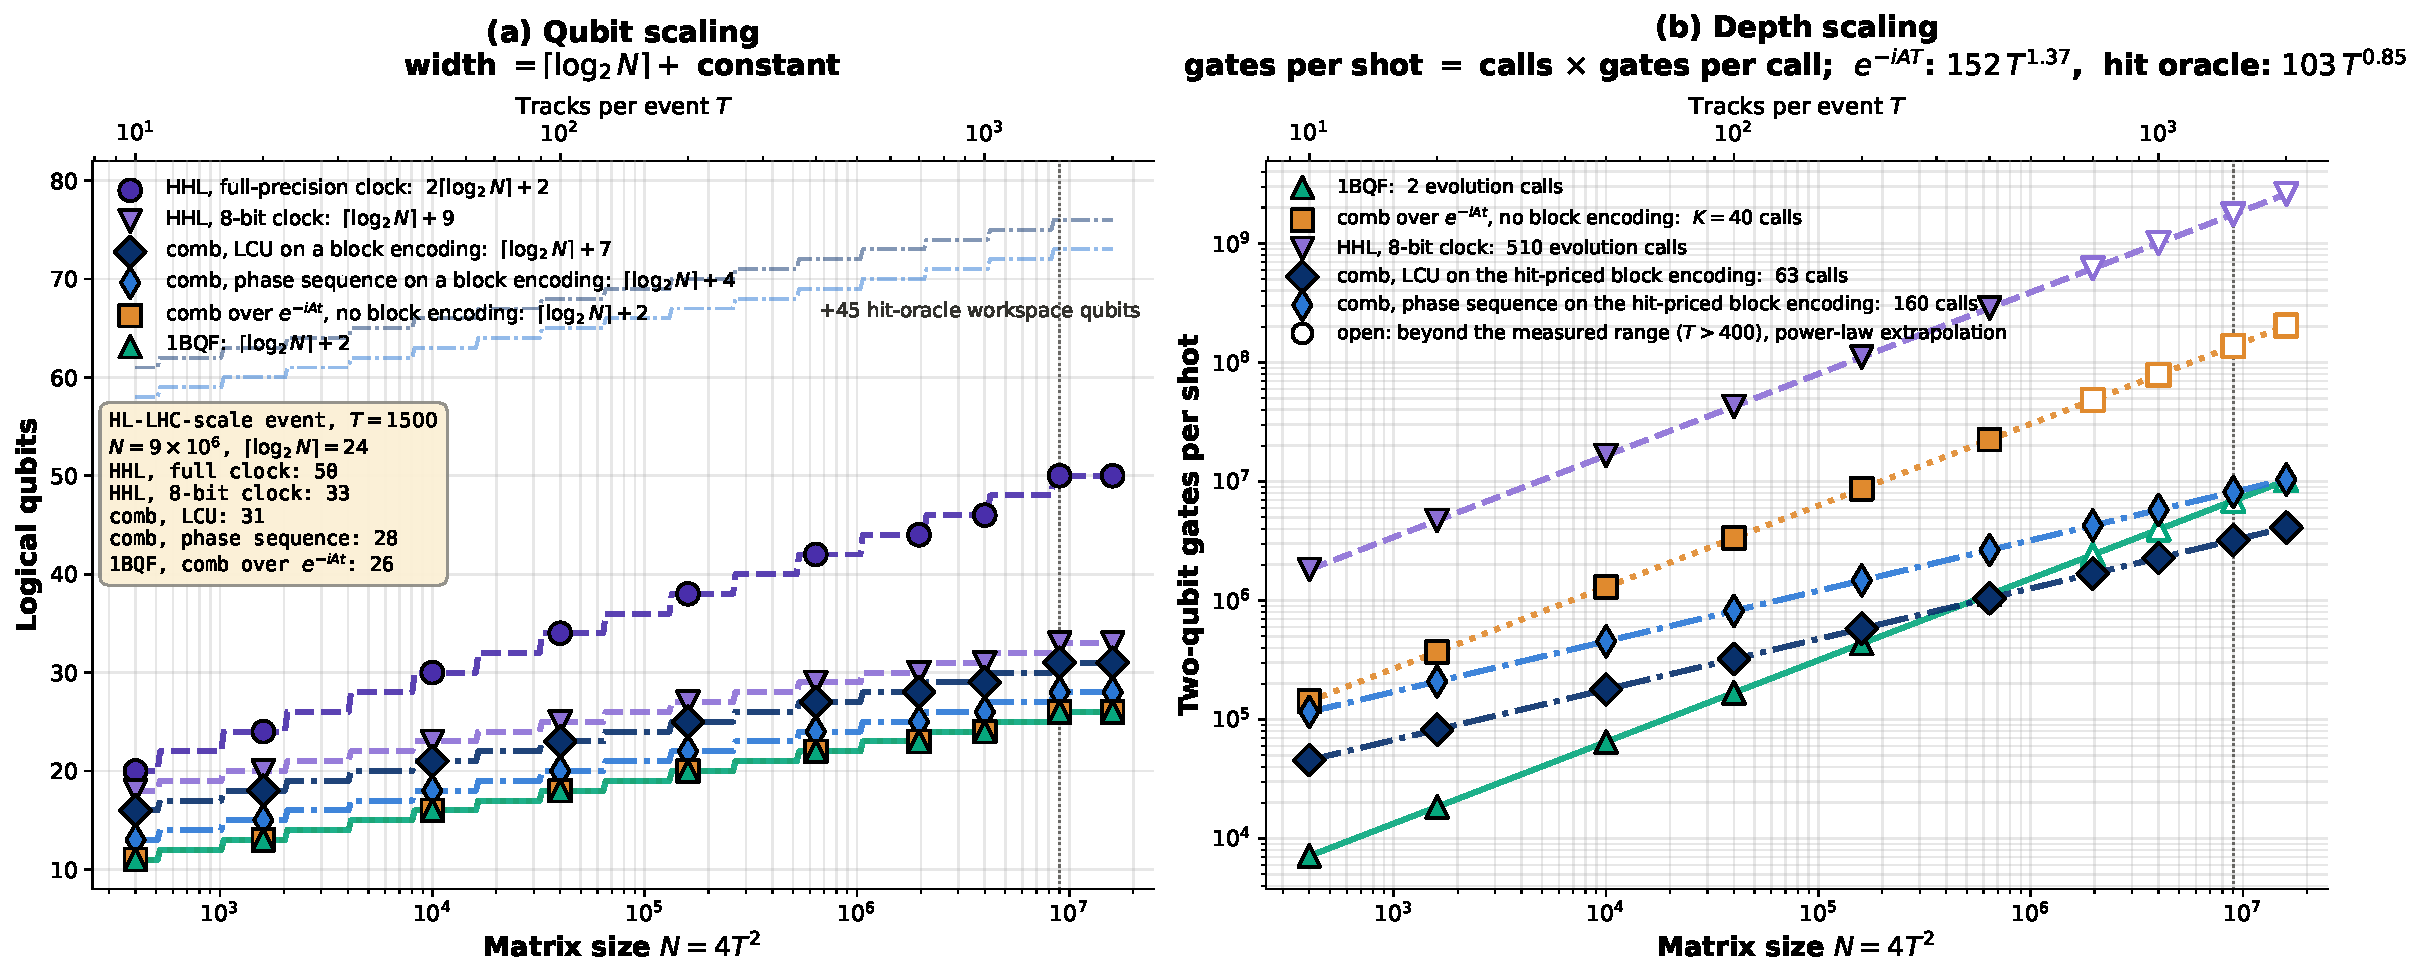
\includegraphics[width=0.98\textwidth]{qubit_scaling.pdf}
\caption{Figure 5. Logical qubits (a) and two-qubit gates per shot (b) against matrix size $N=4T^2$, in the presentation of the predecessor papers; the HL-LHC-scale event at $T=1500$ annotated. Transpiled points to be marked against extrapolated ones; the HHL band labelled as an estimate. \src{fig\_qubit\_scaling, ch.~4.5}}
\end{figure}
\begin{figure}[H]\centering
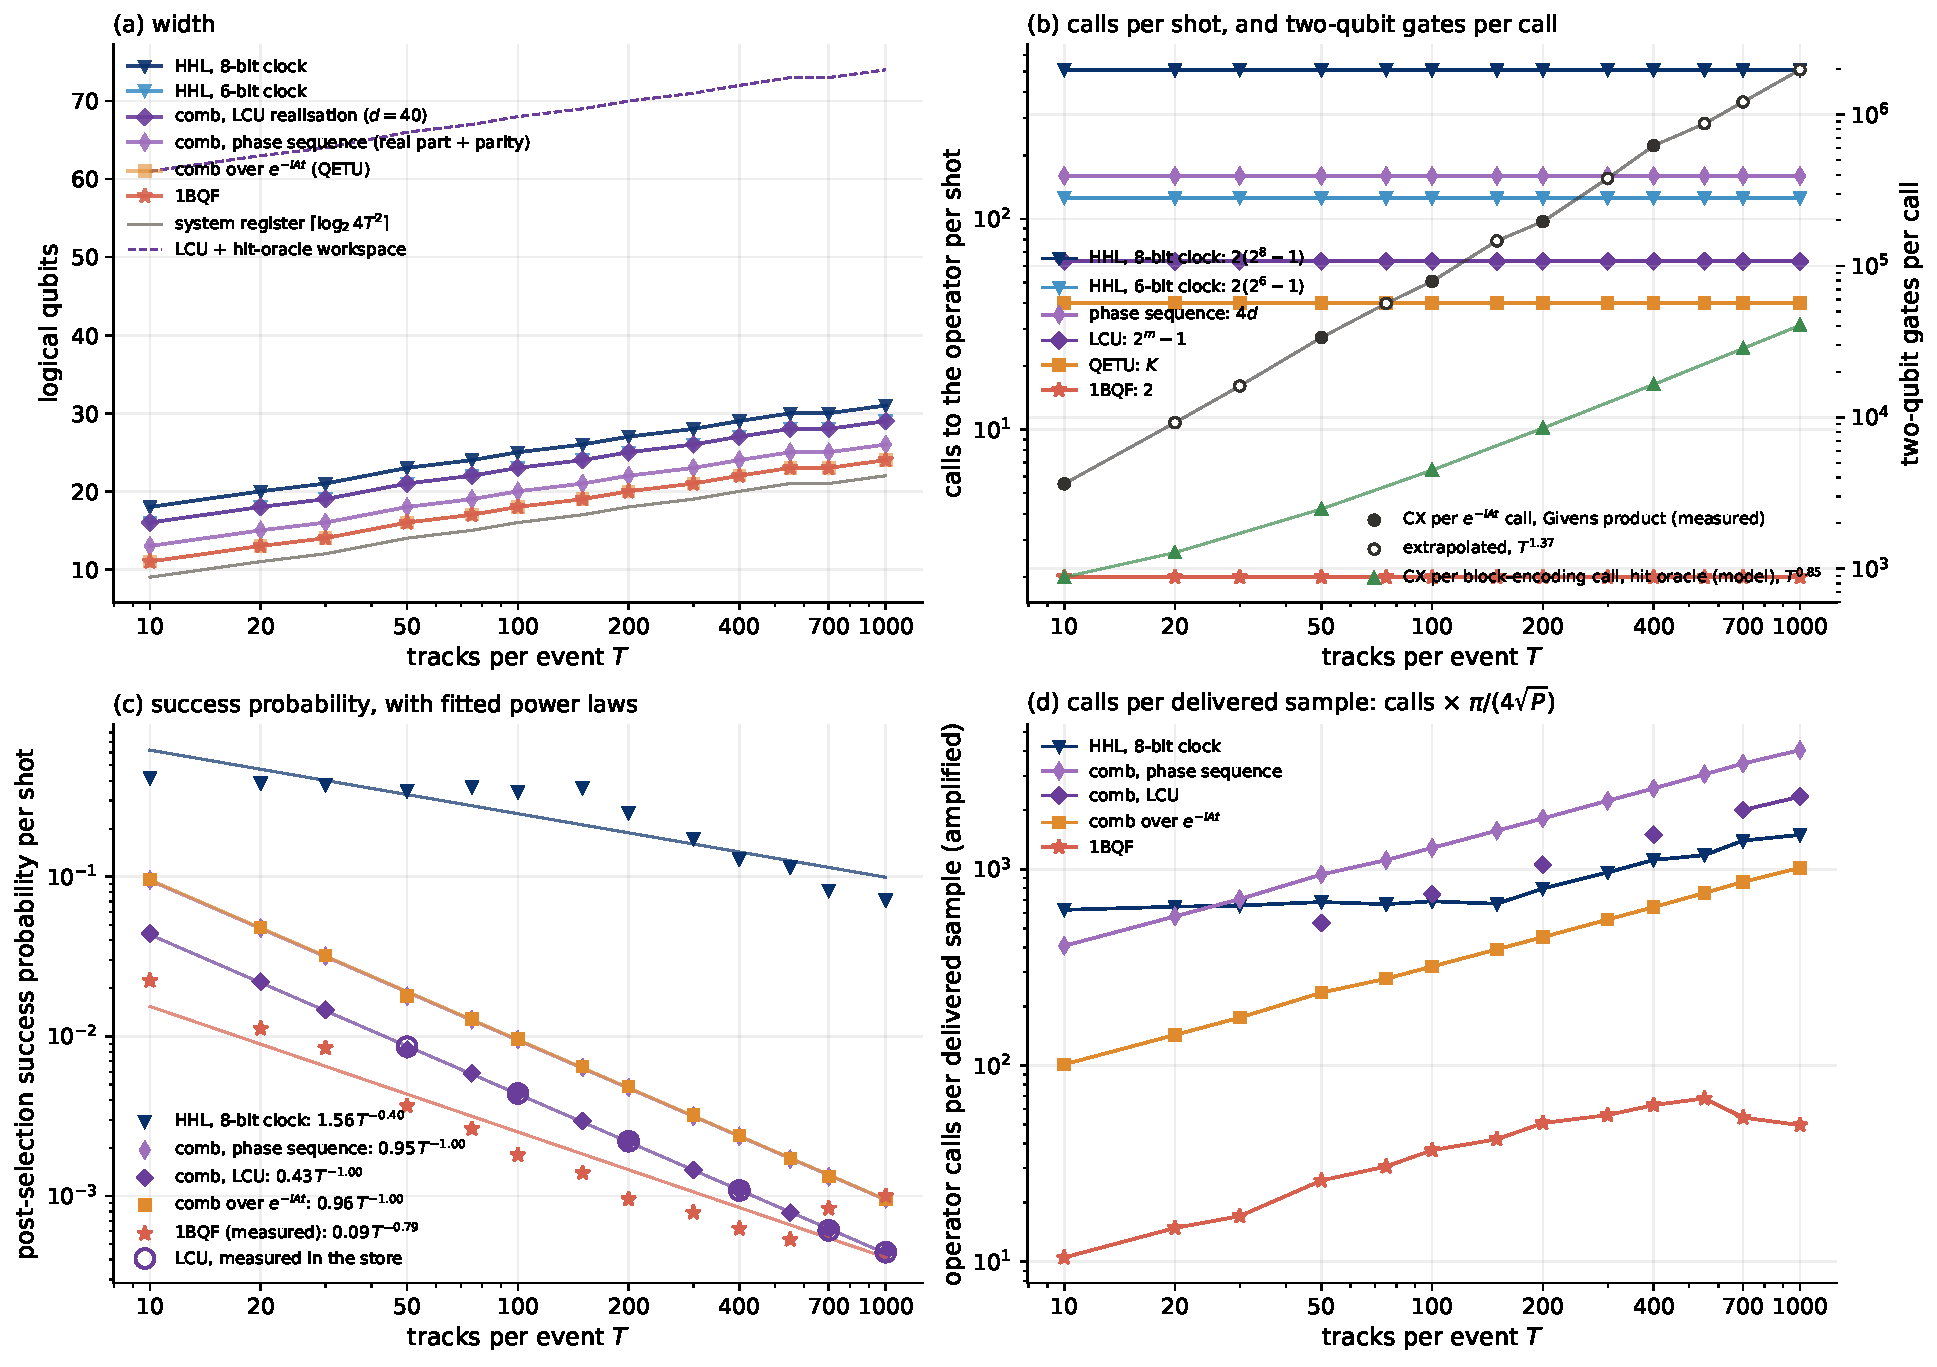
\includegraphics[width=0.55\textwidth]{resource_model.pdf}\hfill
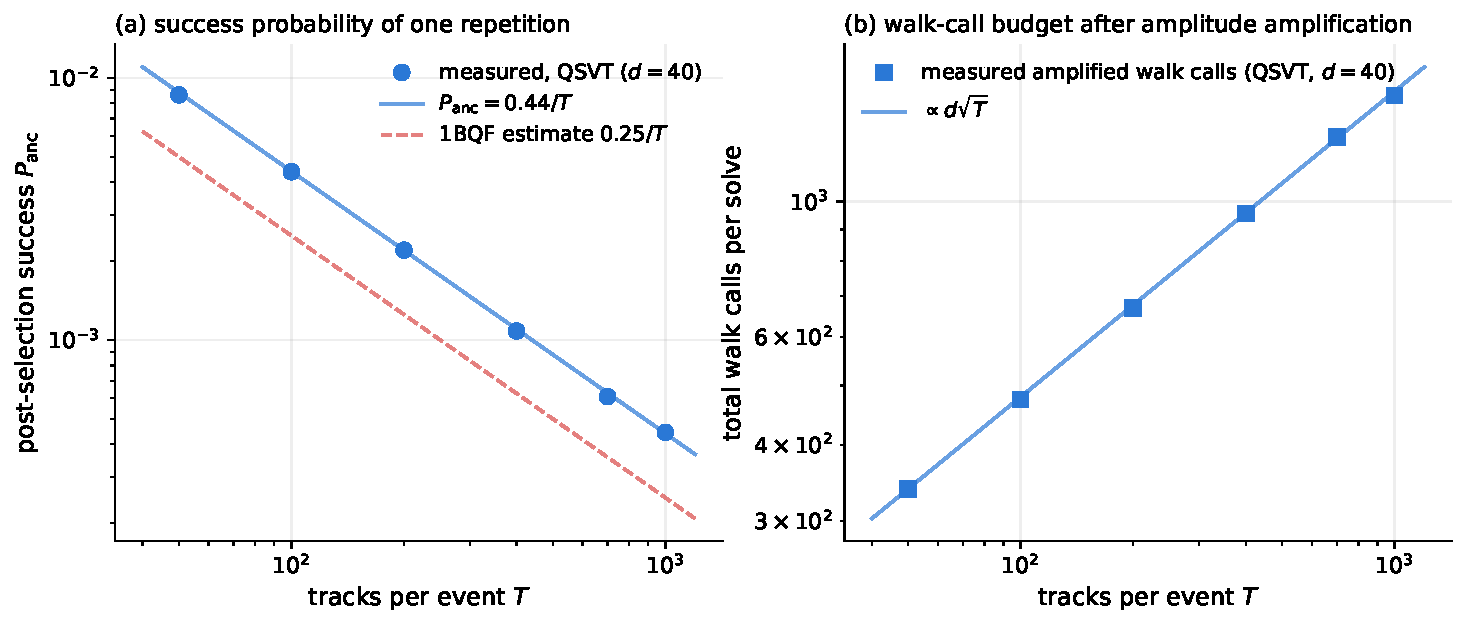
\includegraphics[width=0.42\textwidth]{readout_probability.pdf}
\caption{Figure 6. The five-factor resource model (width, calls, gates per call, amplification, readout) for HHL, the 1BQF and the three comb realisations; the measured post-selection probability and the amplified call budget. \src{fig\_resource\_model, fig\_readout, ch.~4.5, 11.7}}
\end{figure}
\begin{figure}[H]\centering
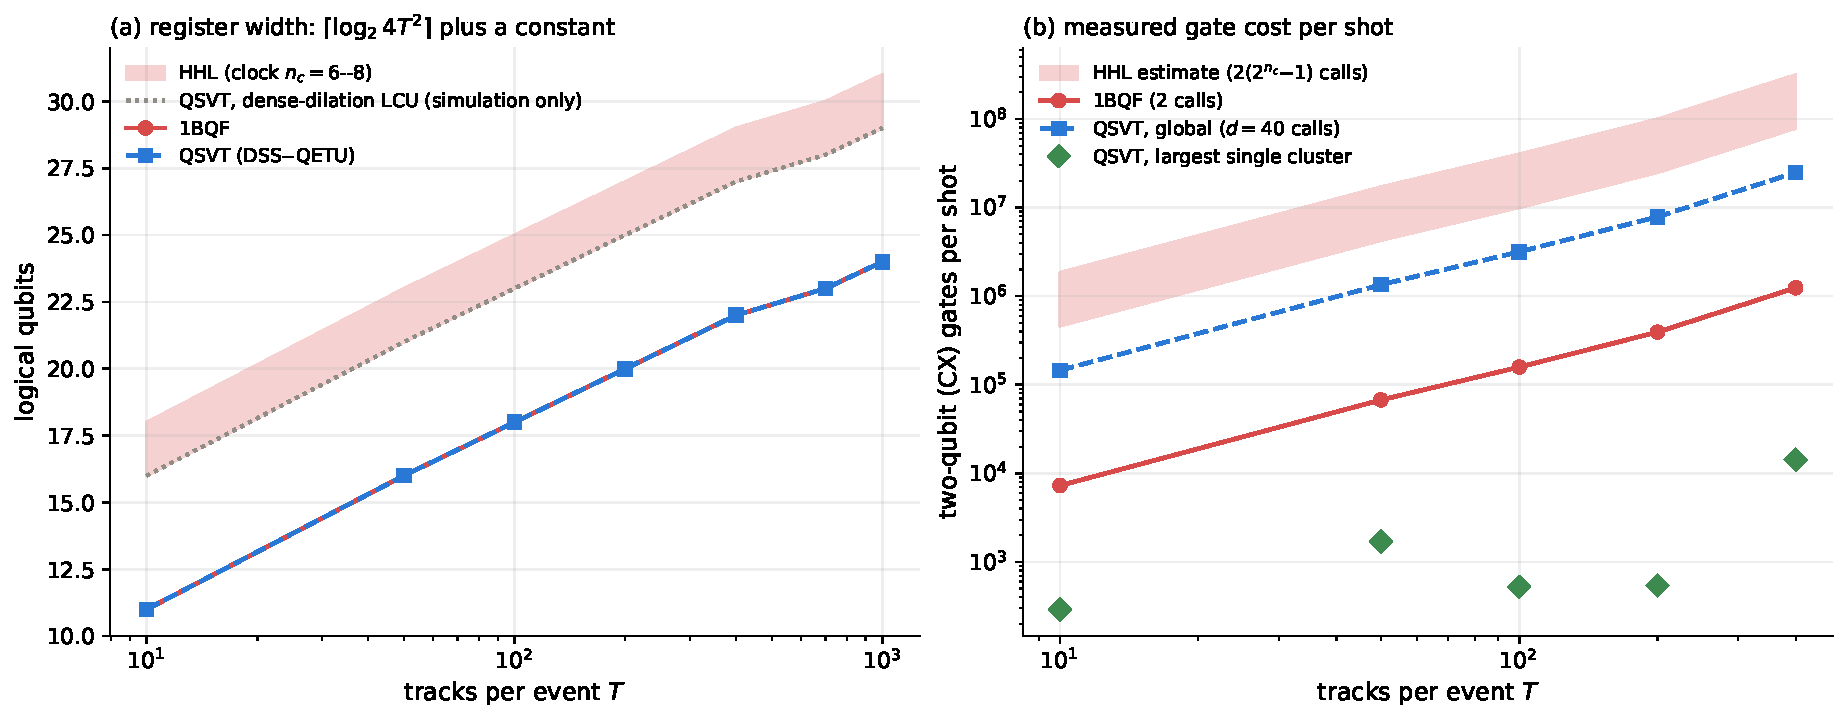
\includegraphics[width=0.9\textwidth]{resource_comparison.pdf}
\caption{Figure 6 (alternative). HHL, the 1BQF and the comb side by side, global and per-cluster routes, with the surface-code estimate. \src{ch.~11.5; HHL is a structure-level estimate}}
\end{figure}
\noindent Numbers: hit oracle $1.6\times10^{4}$ CX per call at $T=400$ against $2.4\times10^{6}$ entry-priced; workspace $+45$--$49$ qubits over the 21-qubit floor; per-cluster comb about $10^{3}$ physical qubits, global comb about $10^{4}$ [ch.~11.5, 11.6]. Classical loading: hit oracle $0.4$\,ms and 8\,KB at $T=400$ (paragraph still to be written).

\section{Outlook}
\msg{Noise moves the false weight onto nameable motif lines and demands a refit (next paper); real geometry turns the lines into a band; the per-cluster route is where this meets hardware; nobody has run QSVT on NISQ hardware, so the algorithm is fault-tolerant by construction.}
\begin{figure}[H]\centering
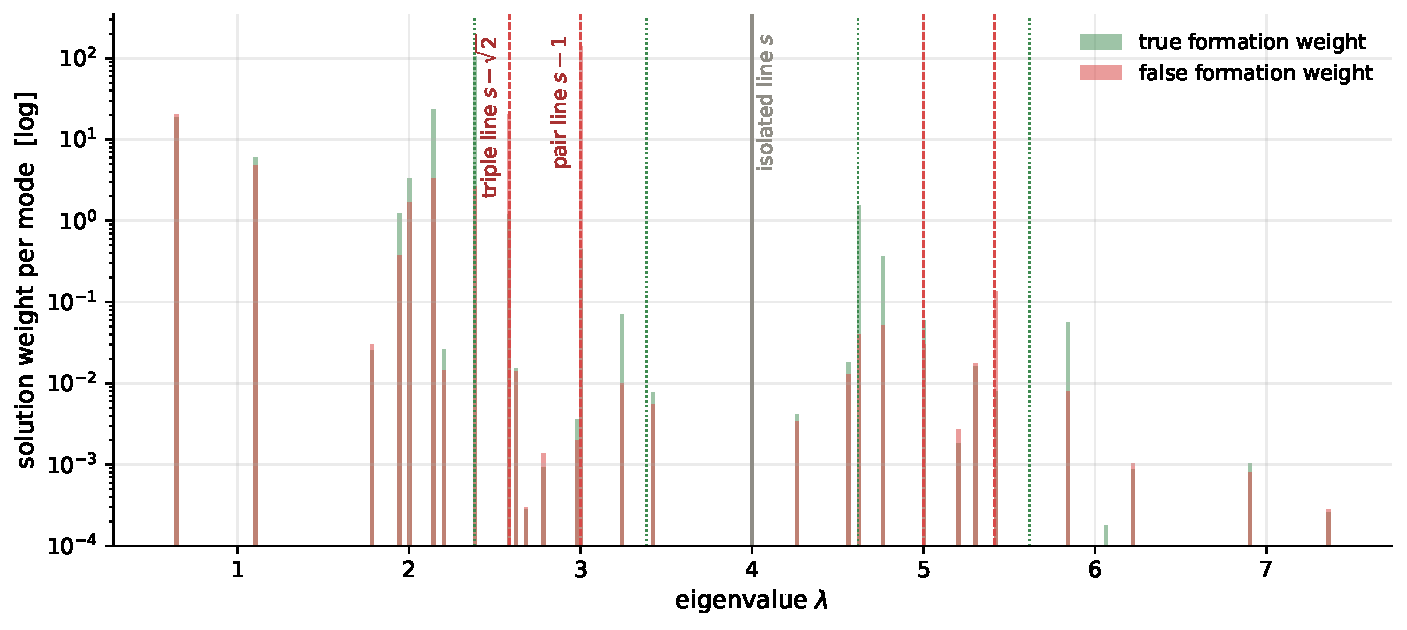
\includegraphics[width=0.55\textwidth]{measured_pileup.pdf}\hfill
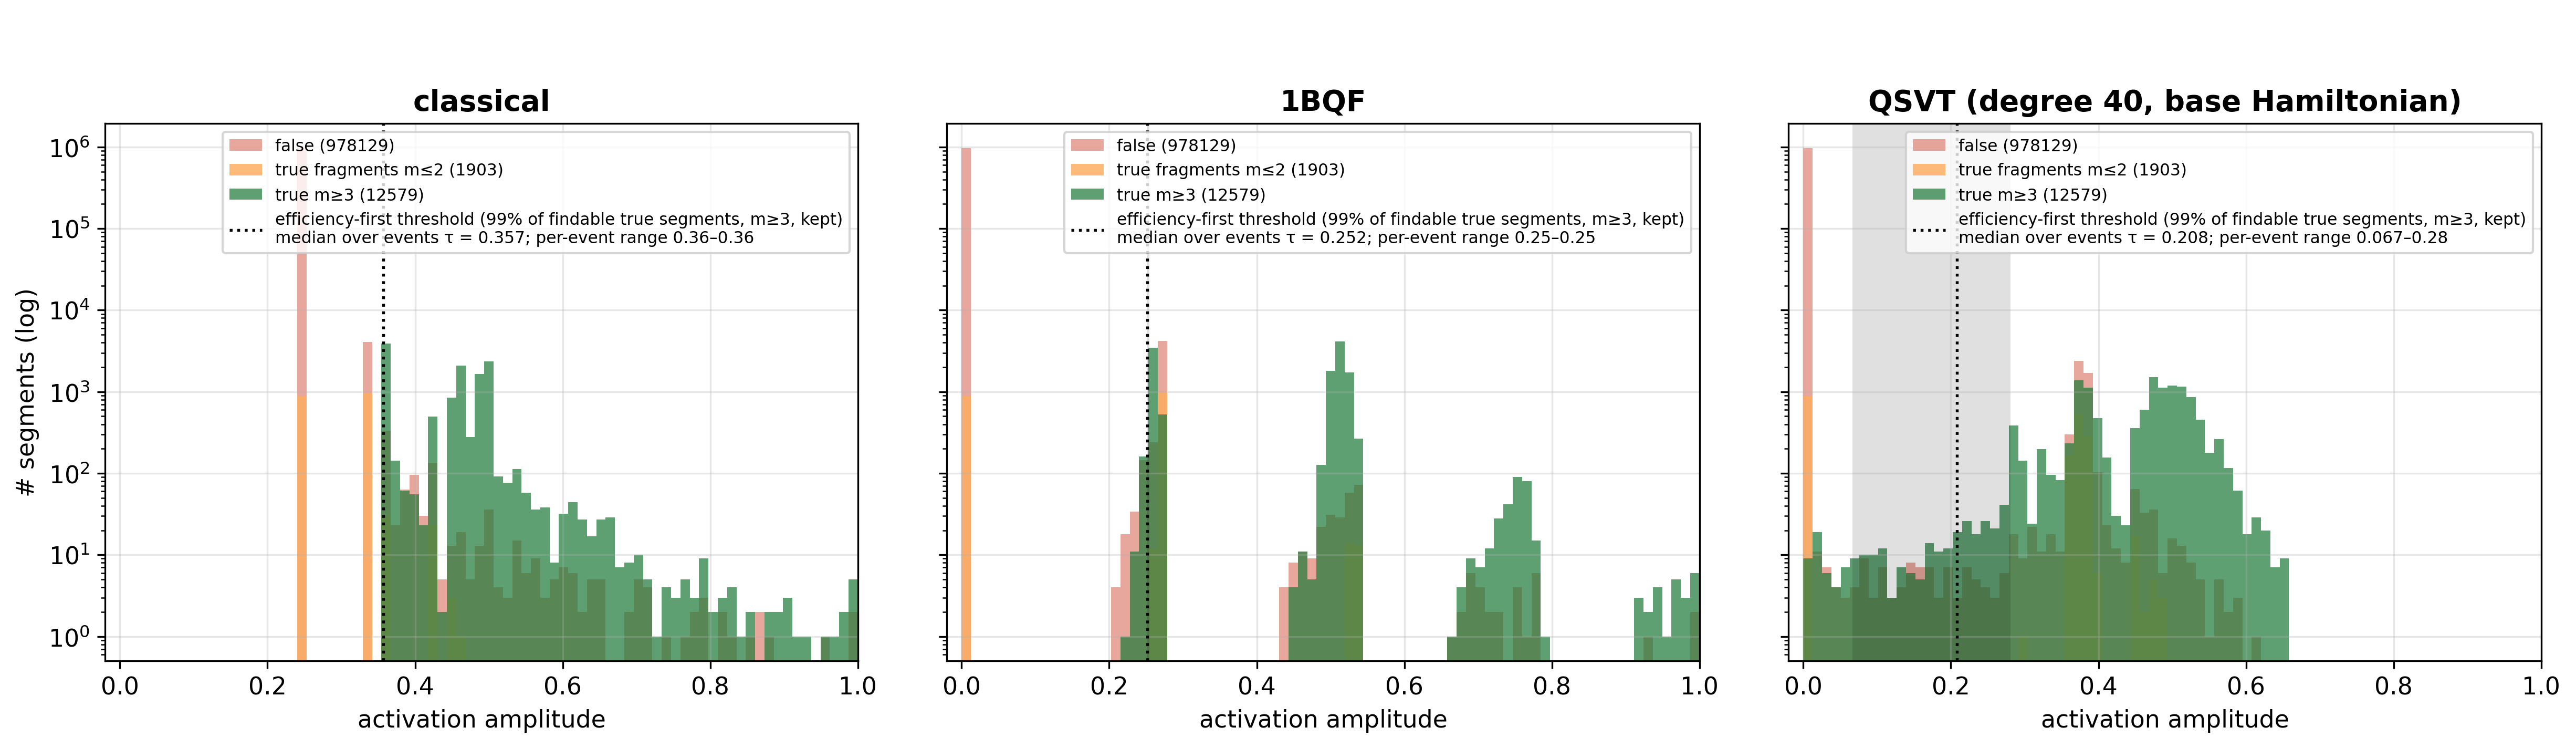
\includegraphics[width=0.42\textwidth]{run3_activation_spectra.png}
\caption{Outlook (optional, one panel at most). The measured false pile-up on the pair and triple lines at heavy noise; activation spectra on real Run-3 geometry, where the true spectrum is a band. \src{ch.~9.1, 11.9}}
\end{figure}

\section*{Methods (stub)}
Events and the noise triple $(\sigma_{\rm scatt},\sigma_{\rm res},\text{hit drop})$ [ch.~2.1]; the acceptance formula above; segment efficiency, false rate and the efficiency-first working point [ch.~2.6]; the shared data pipeline (events and solutions shared segment for segment across the three solvers); the exact simulation chain (explicit circuit, streaming gate sequence, matrix-free semantics, eigendecomposition agree to $10^{-9}$) [ch.~4.4]; which 1BQF object each curve is (exact readout or package circuit).

\section*{Supplement map}
\begin{center}\footnotesize
\begin{tabular}{p{2.1cm}p{2.6cm}p{5.6cm}p{4.6cm}}\toprule
Paper section & Chapter sections & Figure files & Ledger heading \\\midrule
1 Introduction & 1, 3.1, 3.2, 3.6 & circuits.tex; amplitude\_atlas, chain\_amplitude\_ladder & fig:circuits; fig:atlas, fig:ladder \\
2 Spectrum & 2.2, 2.3, 2.4, 2.7 & motif\_gallery; notch\_spectrum & fig\_motifs; fig\_notch\_spectrum \\
3 QSVT & 4.1, 4.2, 4.3, 5.1 & circuits\_qsvt.tex; response\_functions, comb\_degrees & fig:circuitsqsvt; fig\_responses, fig\_comb\_degrees \\
4 Results & 2.6, 5.2, 5.3, 5.5, 10.4 & clean\_headline; spectral\_twins, fragmentation & fig\_clean2x2; fig\_twin, fig\_fragmentation \\
5 Cost & 4.5, 11.5, 11.6, 11.7 & qubit\_scaling; resource\_model, readout\_probability, resource\_comparison & fig\_qubit\_scaling; fig\_resource\_model, fig\_readout; resource\_comparison entry \\
6 Outlook & 6, 11.2, 11.9 & measured\_pileup; run3\_activation\_spectra & (ledger entries of the same names) \\\bottomrule
\end{tabular}
\end{center}
\noindent Held for later papers: the heavy-noise census, the fork and occupancy terms, the refit, the degree and density scans, the transfer problem (paper 3); the block-encoding construction (paper 4); the spectral theorems in proof form (paper 2).
\end{document}
